\begin{frontmatter}
    \begin{abstract}
   Deep generative models, such as Variational Autoencoders (VAEs), are widely used in autonomous driving for learning compact latent representations of input data. However, like other deep neural networks, VAEs are often regarded as black-box models, making it difficult to interpret why a particular decision was made and which attributes contributed to the prediction. This lack of transparency raises concerns about trust and reliability, particularly in safety-critical applications such as autonomous vehicle decision-making. 
   
   One approach to imprioving model interpretability is through counterfactual explanations, which aim to determine the minimal changes required to alter the model's prediction. Counterfactual Explanations provide human-interpretable insights by identifying which features are most influential in a decision, offering an alternative to traditional feature attribution methods. In this work, I propose a novel introspection technique that leverages a deep generative model (VAE) combined with feature masking strategies to generate counterfactual explanations for black-box classifiers. Our approach modifies input images and latent space representations to determine what meaningful changes would lead to a different classification outcome.
   
   To demonstrate the effectiveness of this approach, experiments are conducted using the CARLA dataset, a widely used simulation environment for autonomous driving research. The proposed method allows for a deeper understanding of classifier decisions by revealing how slight modifications in the input or latent representation affect predictions. This work contributes to the broader goal of enhancing transparency and explainability in deep learning models for autonomous systems, addressing the increasing demand for trustworthy AI in real-world applications.
    \end{abstract}

       
    
    \tableofcontents
    % \chapter*{Acknowledgements} % optional
    % I thank my cat Bubbles!
    % \listoffigures % optional
     \listoftables % optional

         % \begin{symbols}
    %     \symbolentry{$\alpha$}{Learning rate, controls the step size during optimization}
    %     \symbolentry{$\gamma$}{Discount factor in reinforcement learning}
    %     \symbolentry{$\theta$}{Model parameters in a neural network}
    %     \symbolentry{$\pi$}{Policy in reinforcement learning}
    %     % Add more symbols as needed
    % \end{symbols}
    
\end{frontmatter}

\chapter{Introduction} \label{Introduction}
\section{Background and Motivation}
Deep neural networks (DNNs) have shown better performance in various domains, such as  image classification~\autocite{s22239544}, medical diagnosis~\autocite{SHAMSHIRBAND2021103627}, natural language processing~\autocite{Wang23}, and autonomous driving~\autocite{s19092064}. However, their fundamental complexity often makes them difficult to interpret, raising concerns over trust and safety. One of the most pressing concern when humans and machines use complex machine learning (ML) models to make crucial decisions, a vital concern is whether humans can trust the model and its predictions. This requirement is must in many fields such as healthcare (for medical treatment decisions), finance (for automated lending decisions), and autonomous vehicles (for decision-making by self-driving cars) where human lives depend on the decisions made by the ML model. Unfortunately, the decisions of such complex models are difficult to explain.

Explainability is the ability to explain the decision-making process of an AI model in terms understandable to the end user~\cite{8631448}. An explainable model provides a clear and intuitive explanation of the decisions made, enabling users to understand why the model produced a particular result. In other words, explainability focuses on why an algorithm made a specific decision and how that decision can be justified.

Recent studies~\cite{Ribeiro2018,chan2022comparativestudyfaithfulnessmetrics,Singh1622975}
 in the domain of explainable ML outline two desired characteristics for explainers: human interpretable i.e., explanations must provide meaningful and qualitative understanding regarding the decision made by the model, by considering human’s limitations, and faithfulness i.e., explanations must correspond to how the model truly behaves. Guided by these desired characteristics, recent research has proposed various methods for explaining ML models. These methods range from feature attribution approaches such as SHAP~\cite{lundberg2017unifiedapproachinterpretingmodel} and LIME~\cite{Ribeiro2018}, example-based approaches such as counterfactual explanations~\cite{wachter2018CE}, and rule-based approaches such as forest-based trees~\cite{SAGI2020124} and DeepRED~\cite{wachter2018CE}.

Deep learning models, in particular, are often referred to as "black boxes" due to their complex, recursive architectures that obscure the reasoning behind their decisions. As the term is presently used in its most common form, an explanation is a separate model that is supposed to replicate most of the behaviour of a black box (for example, ‘the black box says that people who have been delinquent on current credit are more likely to default on a new loan’). Note that the term ‘explanation’ here refers to an understanding of how a model works, as opposed to an explanation of how the world works~\cite{Rudin2019}.

Automated vehicles are promising for decreasing traffic deaths and providing improved mobility, but also pose challenges in addressing the explainability of AI decisions. Autonomous vehicles have to make split-second decisions based on how they classify objects in the scene in front of them. Such misclassifications can lead to dangerous or even fatal outcomes, particularly in real-time safety-critical situations. This is not merely a hypothetical scenario; such incidents are already occurring. For example, a self-driving Uber recently killed a woman in Arizona~\autocite{marshall2019uber}. It was the first known fatality involving a fully autonomous vehicle and a pedestrian. The information reported by anonymous sources claimed that the car software registered an object in front of the vehicle but treated it like a plastic bag or a tumbleweed carried in the wind. This incident underscores the urgent need for explainability in autonomous driving systems, as without a clear understanding of why the model made a particular decision, it is difficult to diagnose errors, improve system reliability, and ensure accountability. Explainable AI methods can provide critical insights into such failures, potentially preventing similar incidents in the future.


The lack of transparency in machine learning models raises significant challenges in domains where explainability is essential for trust and compliance. In safety-critical applications, blindly trusting model predictions is not an option—decisions must be understandable and justifiable. For example, in medical diagnosis, a deep learning model predicting a cancer diagnosis must provide clear reasoning behind its decision to assist doctors in making informed choices. In financial systems, AI models in loan approval processes must explain why an applicant was accepted or rejected to prevent biased decision-making. In security and law enforcement, AI models used for fraud detection or terrorism risk assessment must provide interpretable justifications to ensure fairness and reliability~\autocite{ribeiro2016ML}. An essential criterion for explainable models is that they should bridge the gap between input features and the model’s decision-making process. Ensuring explainability not only enhances trust and user acceptance but also helps in detecting biases, improving system robustness, and meeting regulatory requirements.

Efforts toward explainable AI for autonomous driving have gained momentum, with researchers exploring various interpretability techniques such as saliency maps, attention mechanisms, and rule-based systems~\autocite{bojarski2016endendlearningselfdriving, Ribeiro2018}. However, these approaches often lack actionability. They provide insights into why a decision was made but not how it could have been changed. Counterfactual explanations emerge as a viable approach by identifying the alterations required in input data to yield alternative results. Emerging predominantly in the late 2010s, these explanations aim to provide insights into machine learning decisions by exploring alternative scenarios. They present a human-friendly way to understand complex models \autocite{yeshwanth2023counterfactual}. For example, in the context of autonomous driving, a counterfactual explanation might illustrate how slight adjustments in sensor data, such as images captured by vehicle cameras, could lead to the vehicle stopping rather than proceeding forward. This technique not only offers valuable insights that can improve the model's efficacy and safety but also facilitates a deeper understanding of its decision-making mechanisms. Imagine an autonomous vehicle approaching a pedestrian or dog crossing. The vehicle decides to continue driving, but a counterfactual explanation reveals that if the image data from the camera showed a slightly different configuration of pixels (perhaps indicating the presence of a pedestrian or dog), the model would have decided to stop. This insight could prompt developers to adjust the model to be more sensitive to potential pedestrians, thereby enhancing safety.

By focusing on counterfactual explanation techniques leverages generative models, this thesis seeks to bridge the gap between complex deep learning decisions and human interpretability, with a particular emphasis on safety-critical domains like autonomous driving.

Traditional explanation methods such as LIME and SHAP provide insight into which features influence model decisions, but often fall short in addressing causal reasoning or offering actionable changes. Similarly, gradient-based methods like Integrated Gradients attribute importance but do not indicate how a different outcome might be achieved. Counterfactual explanations address this gap by identifying the minimal changes required to flip a model’s prediction, making them particularly valuable in human-centered, high-stakes applications. Recent work (see \cref{Related work} has explored generating such explanations using generative models in latent space, ensuring realism and plausibility, especially for vision-based tasks like autonomous driving.




\section{Research Objectives}
The primary goal of this research is to develop a framework for generating counterfactual explanations using deep generative models, particularly Variational Autoencoders (VAEs), and to evaluate different feature masking strategies for improving interpretability in autonomous driving systems. This research aims to enhance the explainability of deep learning models by identifying how minimal changes in input features can alter classification outcomes, making AI-driven decisions more transparent and interpretable. Specifically, this research seeks to:

\begin{itemize}
    \item \textbf{Develop a VAE-based framework} for generating counterfactual explanations in deep learning models used in autonomous driving.
    The framework will leverage Variational Autoencoders (VAEs) to learn a latent space representation of input images, enabling the controlled modification of key features to generate counterfactual explanations. The proposed approach will integrate VAEs with a classifier to analyze changes in model predictions when specific latent features are altered. This process will allow for a systematic investigation of how the latent space can be used to generate human-interpretable counterfactuals in an autonomous driving context.

    \item \textbf{Investigate different feature masking techniques and evaluate their effectiveness in counterfactual generation.}  
    This research will explore multiple feature masking strategies to modify/mask input features and analyze their impact on counterfactual explanations. The methods investigated are detailed in the \cref{Methodology} section. The effectiveness of these feature masking techniques will be examined in terms of their ability to produce meaningful and realistic counterfactuals that lead to a change in model prediction.
    
    \item \textbf{Evaluate the counterfactual explanation framework using quantitative metrics.}  
    The generated counterfactuals will be assessed using well-established \textbf{quantitative evaluation metrics} to ensure that they are realistic, structurally similar to the original images, and capable of altering model predictions. These evaluations are clearly explained in \cref{Evaluation and Results}.

    \item \textbf{Conduct a human evaluation study to assess user preferences and interpretability of counterfactual explanations.}  
    Since counterfactual explanations are intended for human understanding, this research will conduct a user study to evaluate the effectiveness of different counterfactual generation techniques from a human perspective. Participants will be shown counterfactual explanations generated by different masking methods and will be asked to select the most preferred counterfactual explanation among different generated alternatives for the same image. They will then be asked to rate each counterfactual explanation based on the common counterfactual metrics like Interpretability, Plausibility, and visual Coherence. The results from this human evaluation will be compared with AI-based quantitative evaluation metrics to determine whether computational assessment aligns with human judgment.

\end{itemize}


\section{Research Questions} \label{sec:research_question}
To achieve the above objectives, this thesis seeks to answer the following key research questions:

\begin{itemize}
    \item \textbf{RQ1:} How can deep generative models be implemented to effectively encode and reconstruct high-dimensional driving scene images for interpretable and compact representation learning in autonomous driving systems?

    \item \textbf{RQ2:} How can loss function modifications in Variational Autoencoders (VAEs) optimize image reconstruction quality in autonomous driving tasks? 
    
    \item \textbf{RQ3:} How do different masking techniques impact the effectiveness and efficiency of counterfactual explanation generation, in terms of coverage, computational cost, method overlap, and failure rate?  (See \cref{Methodology} for details on the techniques investigated.) 

    \item \textbf{RQ4:} Which counterfactual explanation method is most preferred by users when selecting among generated explanations of the same original image? What factors influence user preference? (See \cref{Methodology} for details on the methods compared.)
\end{itemize}

\section{Thesis Structure (Outline of Chapters)}
This thesis is organized into multiple chapters, each addressing a key aspect of the research. \autoref{Introduction} introduces the motivation behind this work, outlines the problem statement, research objectives and questions, and provides an overview of the thesis structure. The
\autoref{Background} covers foundational concepts. It also introduces relevant evaluation metrics and properties and also applications.
The \autoref{Methodology} presents the core methodological contributions of the thesis. It details the dataset collection, the architecture and training process of the VAE and classifier, various feature masking techniques, and the process for generating counterfactual explanations. The \autoref{Evaluation and Results} reports both AI-based and human-centered evaluations. It presents different metrics and results, followed by an in depth user study and concludes with the overall discussion. The \autoref{Related work} chapter situates this thesis within the context of existing literature by reviewing and comparing prior work by other researchers. It highlights the key contributions of previous studies, identifies research gaps, and explains how this thesis builds upon and extends those works. Furthermore, it discusses how inspiration was drawn from existing methods and how this research addresses the identified limitations. Finally, \autoref{Conclusion and Future Scope} summarizes the key contributions, discusses limitations, and outlines potential directions for future research.

\chapter{Background} \label{Background}
This section introduces notations and provides background on counterfactual explanations, Variational Autoencoders, LIME, Classifiers, and CARLA.

\section{Counterfactual Explanations}
In machine learning, decisions are often made by complex models without explicit explanations. For instance, imagine an autonomous vehicle approaching an intersection, relying on its vision system to classify traffic signs. If the vehicle recognizes a STOP sign, it will halt; however, if it misclassifies the same sign as a Speed Limit sign, this might lead to undesired consequences. Understanding precisely what minimal changes to the input would alter the model's decision is critical. This concept is precisely captured by \textit{counterfactual explanations}.

Formally, following Molnar~\cite{molnar2024}, a counterfactual explanation identifies the smallest possible modification to an input instance resulting in a different prediction outcome. Given a black-box classifier \( b \) that predicts an outcome \( y \) for an input instance \( x \):

\begin{equation}
y = b(x),
\end{equation}

a \textit{counterfactual explanation} finds an alternative instance \( x' \), such that:

\begin{equation}
b(x') \neq b(x),
\end{equation}

with the condition that the difference between \( x \) and \( x' \) is minimized according to a suitable distance metric.

For instance, in autonomous driving, if the classifier originally labels an image as:

\begin{equation}
b(x) = \text{"STOP Sign"},
\end{equation}

a valid and realistic counterfactual might suggest a slight reduction of brightness by 10\%, resulting in:

\begin{equation}
b(x') = \text{"Speed Limit Sign"}.
\end{equation}

\subsection{Desirable Properties of Counterfactual Explanations} \label{subsec:background_desirable_properties_of_CEs}
Counterfactual explanations are evaluated based on several key desirable properties~\cite{guidotti2022counterfactual}, each ensuring usefulness, interpretability, and practicality:

\begin{enumerate}
    \item \textbf{Validity:}  
    Validity measures the proportion of generated counterfactuals that achieve the desired classification change:
    \begin{equation}
        b(x') \neq b(x).
    \end{equation}
    A higher validity score is preferable, indicating effective counterfactual generation.

    \item \textbf{Proximity (Minimality of Change):}  
    Counterfactual changes should be minimal, measured by a distance function \( d(x, x') \):
    \begin{equation}
        d(x, x') \text{ is minimized, with } d(x,x') < \delta,
    \end{equation}
    where \( \delta \) is a predefined threshold. Commonly used metrics include:
    \begin{itemize}
        \item \textbf{L1 norm (MAE)}: Sum of absolute differences.
        \item \textbf{L2 norm (MSE)}: Sum of squared differences.
        \item \textbf{Logcosh loss \cite{chen2019log}}: Smooth variant of MSE.
    \end{itemize}

    For instance, in autonomous driving, realistic counterfactual modifications involve adjusting brightness or contrast without changing essential features like the shape or position of a traffic sign. Lower values for proximity metrics indicate better counterfactual explanations.

    \item \textbf{Plausibility (Realism):}  
    Counterfactual instances must remain realistic and consistent with the original data distribution. For instance, suggesting a triangular STOP sign would be implausible since STOP signs are universally octagonal.

    \item \textbf{Actionability:}  
    Counterfactual recommendations must suggest feasible and realistic actions. For instance, suggesting increasing income or clearing existing debts is actionable for loan approval scenarios, whereas altering immutable features like age or gender is neither practical nor ethical.
\end{enumerate}



\subsection{Desirable Properties of Counterfactual Explainers}
A counterfactual explainer is the algorithm or system responsible for generating counterfactual instances. In evaluating such explainers, especially in safety-critical domains like autonomous driving, certain properties are considered desirable. While many of these properties have been proposed in the broader XAI literature~\cite{guidotti2022counterfactual, DELANEY2023103995}, in this thesis we focus on those directly measurable and relevant to our proposed masking-based methods.

\begin{itemize}
    \item \textbf{Effectiveness:} The ability to consistently generate valid counterfactuals across all classes. The more effective the explainer the more industries prefer the algorithm to implement in real time.

    \item \textbf{Efficiency} refers to the computational time and resources needed to generate explanations. For real-time interpretability in autonomous systems, fast generation is critical.

    \item \textbf{Semantic Targeting:} A good explainer should modify only the causal parts of the image or latent representation.

    \item \textbf{Sparsity} and \textbf{Minimality} concern how many features are modified in generating a counterfactual. Explanations that introduce fewer changes are easier for humans to understand and are more interpretable.
\end{itemize}

\subsection{Evaluation Metrics for Counterfactual Generation Algorithms}
Most counterfactual generation algorithms are evaluated based on the desirable properties mentioned above. Although the ideal evaluation would involve a user study to assess real-world usability, research typically uses quantifiable metrics instead~\cite{Singh1622975, DBLP:journals/corr/abs-2010-10596, wang2024counterfactual}. Common quantitative evaluation metrics include:

\begin{itemize}
    \item \textbf{Validity}: Validity measures the ratio of counterfactuals that actually achieve the desired class label to the total number of counterfactuals generated. This metric is fundamental as it assesses whether the counterfactual successfully flips the prediction to the target class. Without validity, a counterfactual explanation fails its primary purpose of showing how an alternative outcome could be achieved.
    \item \textbf{Proximity:} Average distance between original and counterfactual instances, typically measured using L1, L2 norms, or similar metrics.
    \item \textbf{Plausibility:} Assessment of realism within the data distribution (e.g., reconstruction error using VAEs or distance to nearest neighbors) Typically measured using distance metrics like L1 (Manhattan) or L2 (Euclidean) norms.
    \item \textbf{SSIM:} For image-based counterfactual explanations, SSIM provides a perceptually aligned method for measuring similarity between original and counterfactual images. Unlike simple pixel-wise comparisons, SSIM identifies structural information and measures the differences between this information extracted from the two images. 
\end{itemize}

These metrics provide a systematic and practical way to assess the quality of generated counterfactual explanations. These properties will be empirically assessed in \cref{Evaluation and Results} section~\ref{sec:masking_eval}.





















\section{Variational Autoencoders (VAE) for Representation Learning}
Generative modeling is an area of machine learning aimed at creating models capable of capturing and modeling complex probability distributions from observed datasets~\cite{doersch2016tutorial}. The overarching goal is to learn the underlying structure and dependencies of data, which is particularly useful in high-dimensional scenarios like images. For instance, in image generation, a generative model must understand intricate pixel-level relationships to produce realistic samples.

Variational Autoencoders (VAEs) represent a significant advancement in generative modeling by combining deep learning with principles from Bayesian inference. VAEs learn a probabilistic mapping from high-dimensional data to a structured latent space, facilitating both representation learning and data generation. This section provides an in-depth discussion of VAEs, covering their theoretical foundations, latent variable modeling, and applications.

\subsection{From Regular Autoencoders to Variational Autoencoders}
Traditional autoencoders (AEs) are designed to learn efficient low-dimensional representations of input data through a deterministic encoding-decoding process. The encoder compresses input data into a fixed-dimensional latent space, and the decoder reconstructs the original input from this compressed representation. While effective for feature extraction and data compression, traditional autoencoders lack a well-defined probabilistic structure, limiting their ability to generate diverse and novel samples. Variational Autoencoders (VAEs) address this limitation by introducing a probabilistic approach, where each input is mapped to a distribution in the latent space rather than a single point. This enables VAEs to generate new, meaningful samples by sampling from the learned latent distribution, making them powerful generative models.

\subsection{Foundations of Variational Autoencoders}
Variational Autoencoders, introduced by Diederik P. Kingma and Max Welling in their seminal 2013 paper~\cite{kingma2022autoencodingvariationalbayes} revolutionized the field of generative modeling. Unlike traditional autoencoders that primarily focus on data compression and reconstruction, VAEs remarkable ability to generate new data that resembles the training distribution. This capability stems from their unique approach to latent space representation, where inputs are mapped to probability distributions rather than fixed points. 

A VAE consists of two primary components: a probabilistic encoder and a probabilistic decoder. The encoder compresses input data into a latent representation, while the decoder reconstructs the original data from the latent variables. These two components are parameterized as neural networks and optimized using a variational inference approach.

\subsection{Variational Inference: An Approximate Inference Method} 
Variational inference is a technique used in Bayesian statistics and machine learning to approximate intractable posterior distributions. In the context of VAEs, it is employed to approximate the true posterior distribution $p(z|x)$ of the latent variables given the observed data $x$, since direct computation is intractable. Instead of computing the exact posterior, VAEs introduce an approximate distribution $q_\phi(z|x)$, which is parameterized by the encoder network. The objective of variational inference is to find the optimal parameters $\phi$ such that $q_\phi(z|x)$ closely resembles the true posterior $p(z|x)$. This is achieved by minimizing the Kullback-Leibler (KL) divergence between the two distributions:
\begin{equation}
D_{KL}(q_\phi(z|x) || p(z|x)) = \mathbb{E}{q\phi(z|x)}[\log q_\phi(z|x) - \log p(z|x)].
\end{equation}
Since directly computing $p(x)$ is computationally expensive, variational inference instead maximizes the Evidence Lower Bound (ELBO), which is a surrogate objective that indirectly minimizes the KL divergence. By optimizing the ELBO, VAEs effectively learn to generate meaningful latent representations while ensuring that the approximate posterior remains close to the true posterior.

\subsection{Directed Probabilistic Models and Latent Variables}

VAEs are grounded in the framework of directed probabilistic models, commonly known as Bayesian networks. These models employ a directed acyclic graph (DAG) to represent dependencies among random variables. In VAEs, the generative process is modeled using a probabilistic graphical representation, where a latent variable $z$ is assumed to generate the observed data $x$.

Given an observed dataset $X = {x_1, x_2, ..., x_N}$, we assume that each data point $x_i$ is generated by a corresponding latent variable $z_i$. The generative process is characterized by a prior distribution over latent variables $p(z)$ and a likelihood model $p(x|z)$:
\begin{equation}
p(x) = \int p(x|z) p(z) dz.
\end{equation}
Since computing the exact posterior $p(z|x)$ is intractable due to the complexity of integrating over the latent space, VAEs leverage variational inference to approximate this posterior with a tractable distribution $q_\phi(z|x)$ parameterized by an encoder network.

\subsection{Variational Inference and the Evidence Lower Bound (ELBO)} \label{sec:variational_inference}
To approximate the posterior $p(z|x)$, VAEs introduce a variational distribution $q_\phi(z|x)$, typically chosen as a Gaussian distribution with mean $\mu_\phi(x)$ and variance $\sigma^2_\phi(x)$. The objective is to make $q_\phi(z|x)$ as close as possible to the true posterior by minimizing their Kullback-Leibler (KL) divergence~\cite{stackexchange_kl_vae}:
\begin{equation}
D_{KL}(q_\phi(z|x) || p(z|x)) = \mathbb{E}{q\phi(z|x)}[\log q_\phi(z|x) - \log p(z|x)].
\end{equation}
Since directly computing $p(x)$ is intractable, we maximize the Evidence Lower Bound (ELBO) instead:
\begin{equation}
\log p(x) \geq \mathbb{E}{q\phi(z|x)}[\log p_\theta(x|z)] - D_{KL}(q_\phi(z|x) || p(z)).
\end{equation}
The ELBO consists of two terms: a reconstruction term, which ensures that the decoded data resembles the input, and a regularization term, which encourages the approximate posterior $q_\phi(z|x)$ to be close to the prior $p(z)$. The prior is typically chosen as a standard normal distribution $\mathcal{N}(0, I)$ for simplicity and computational efficiency.


\subsection{Structure of Variational Autoencoders}
Figure \ref{fig:vae_structure} provides a schematic representation of the VAE architecture. A VAE comprises three main components:

\begin{figure}[htbp]
    \centering
    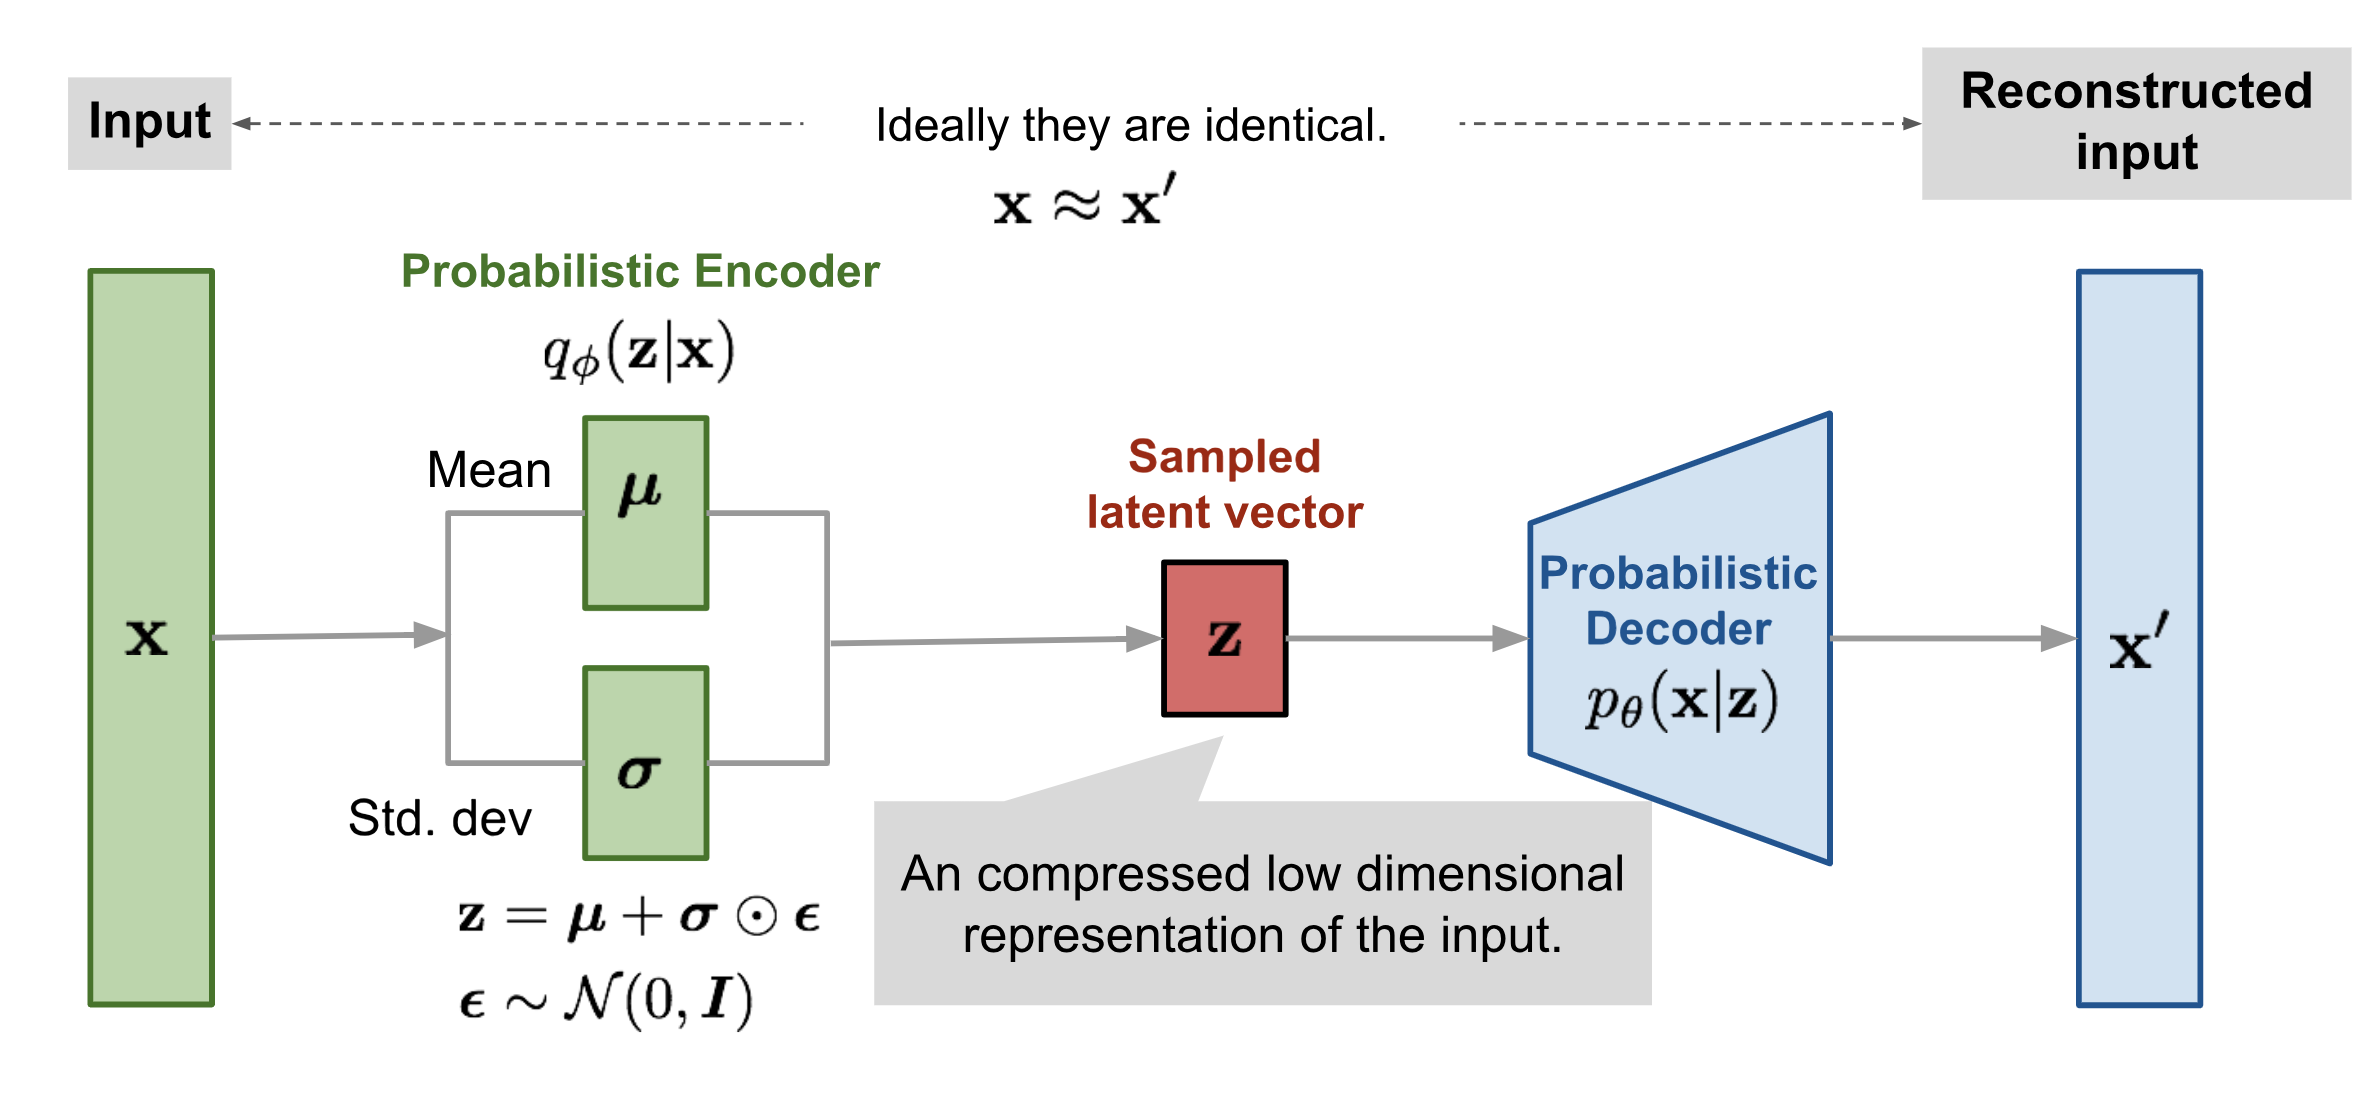
\includegraphics[width=0.7\textwidth]{img/vae/vae-gaussian.png}
    \caption[Architecture of a Variational Autoencoder (VAE)]{Architecture of a Variational Autoencoder (VAE). The encoder maps inputs to a latent distribution; the decoder reconstructs data from samples drawn from this distribution~\cite{weng2018VAE}.}
    \label{fig:vae_structure}
\end{figure}

\subsubsection{Encoder}
The encoder network maps input data  to a lower-dimensional latent space . Unlike traditional autoencoders, the encoder of a VAE outputs parameters defining a probabilistic distribution in latent space. Specifically, the encoder produces vectors representing the mean  and variance  for each latent dimension, defining a multivariate Gaussian distribution:
\begin{equation}
q(z|x) = \mathcal{N}(z; \mu(x), \Sigma(x)), \quad \text{where } \Sigma(x) = \text{diag}(\sigma_1^2, \dots, \sigma_n^2).
\end{equation}
\begin{figure}[htbp]
    \centering
    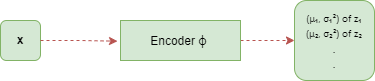
\includegraphics[width=0.7\textwidth]{img/vae/Image To Encoder To Latent Variable Parameters.png}
    \caption[Encoder network mapping input to latent parameters]{Encoder network ($\phi$) mapping input $x$ to latent space parameters $(\mu_i, \sigma_i^2)$ for each latent dimension $z_i$. The encoder learns the approximate posterior distribution $q(z|x) = \mathcal{N}(z; \mu(x), \Sigma(x))$.}
    \label{fig:encoder}
\end{figure}

\subsubsection{Latent Variables}
Latent variables  are unobserved abstract representations inferred from the data during training. These variables provide a compressed, lower-dimensional abstraction of the data, capturing its essential features.

\subsubsection{Decoder}
The decoder reconstructs input data  from latent variables . It is designed probabilistically, modeling the conditional distribution . This setup allows the decoder to generate new data points resembling those from the training set by sampling from the latent distribution.
\begin{figure}[htbp]
    \centering
    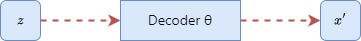
\includegraphics[width=0.7\textwidth]{img/vae/decoder_figure.png}
    \caption[Decoder network reconstructing outputs from latent space]{Decoder network ($\theta$) mapping latent variables $z$ to reconstructed output $x'$. The decoder models the likelihood $p(x'|z) = \mathcal{N}(x'; \mu_\theta(z), \sigma_\theta^2(z))$.}
    \label{fig:decoder}
\end{figure}


\subsection{VAE Objective Function and Loss} \label{subsec:VAE Objective Function and Loss}
The training objective of VAEs, derived from variational inference, maximizes the Evidence Lower Bound (ELBO):
\begin{equation}
\log p(x) \geq \mathbb{E}{q(z|x)}[\log p(x|z)] - D{KL}(q(z|x) \parallel p(z)).
\end{equation}

The first term is the reconstruction likelihood, encouraging accurate data reconstruction, while the second term ensures the approximate distribution  closely resembles the prior . Typically, a unit Gaussian  serves as the latent prior.

\subsection{Reparameterization Trick} \label{subsec:reparameterization_trick}
Training VAEs involves optimizing stochastic processes that require backpropagation, making direct sampling problematic. The "reparameterization trick" addresses this by decoupling randomness from network parameters. Instead of sampling directly from the learned latent distribution \( z \sim \mathcal{N}(\mu(x), \sigma^2(x)) \), we sample from a standard normal distribution and transform it using the mean and standard deviation produced by the encoder network:
\begin{equation}
z = \mu(x) + \sigma(x) \odot \epsilon, \quad \text{where } \epsilon \sim \mathcal{N}(0, I).
\end{equation}
This reparameterization allows gradients to propagate through the sampling process, enabling efficient end-to-end optimization via backpropagation.


As illustrated in Figure~\ref{fig:reparameterization_trick}, the reparameterization trick decomposes the sampling process into deterministic and stochastic components. The encoder network predicts the mean \( \mu(x) \) and standard deviation \( \sigma(x) \) of the latent Gaussian distribution. A latent vector \( z \) is then obtained by sampling a noise vector \( \epsilon \sim \mathcal{N}(0, I) \) and applying the transformation:
\[
z = \mu(x) + \sigma(x) \odot \epsilon.
\]
This formulation preserves the stochastic nature of the latent space while allowing the sampling operation to remain differentiable, enabling gradient-based optimization through backpropagation.


Furthermore, Figure \ref{fig:reparameterization_backprop} demonstrates how the reparameterization trick enables backpropagation through stochastic nodes. Since the sampling operation is reformulated as a differentiable function of the noise variable , gradients can flow backward through  and , allowing efficient learning of the latent distribution parameters. This ensures that the encoder network effectively learns a structured latent space while maintaining a probabilistic formulation.

\begin{figure}[htbp]
    \centering
    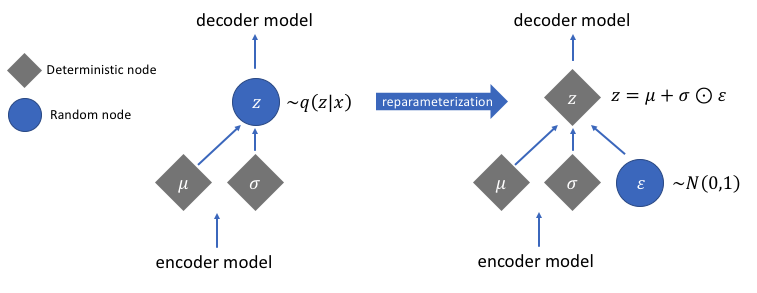
\includegraphics[width=0.6\textwidth]{img/vae/reparameterization_trick.png}
    \caption[Reparameterization trick visualization]{Visualization of the reparameterization trick: converting stochastic sampling into deterministic operations for effective backpropagation. Source: Kingma and Welling~\cite{Kingma_2019}.}
    \label{fig:reparameterization_trick}
\end{figure}

\begin{figure}[htbp]
    \centering
    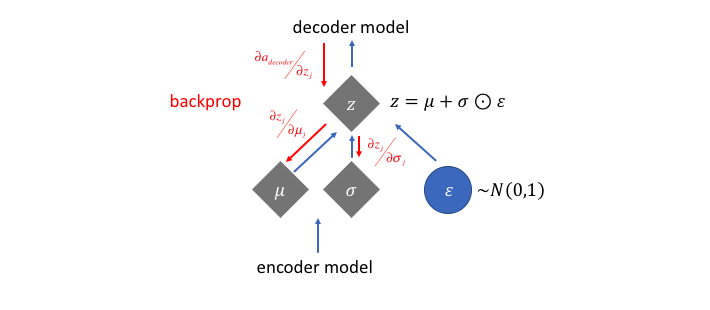
\includegraphics[width=0.7\textwidth]{img/vae/reparameterization_backprop.png}
    \caption[Backpropagation flow via reparameterization trick]{Illustration of gradient flow (backpropagation) enabled by the reparameterization trick in VAEs. Source: Kingma and Welling~\cite{Kingma_2019}.}
    \label{fig:reparameterization_backprop}
\end{figure}


This transformation allows gradients to flow smoothly through the stochastic layers, enabling effective optimization.






\subsection{Applications of Variational Autoencoders}
VAEs have broad applicability across various domains:

\begin{itemize}
\item \textbf{Image Generation}: Creating new synthetic images with controlled variations.
\item \textbf{Data Denoising}: Removing noise from data by reconstructing from a clean latent representation.
\item \textbf{Dimensionality Reduction}: Compressing high-dimensional data into lower-dimensional representations for analysis and visualization.
\item \textbf{Anomaly Detection}: Identifying outliers by assessing reconstruction errors.
\end{itemize}

In summary, Variational Autoencoders bridge deep learning with probabilistic graphical models, allowing sophisticated representation learning and powerful generative capabilities, especially when handling complex, high-dimensional data like images.


















\section{Post-hoc Explainability Methods (LIME)}

Post-hoc methods are explainability techniques applied \textit{after} a model has made a prediction to understand the decision-making process. Unlike inherently interpretable models such as decision trees, many deep learning (DL) and machine learning (ML) models act as black boxes. Post-hoc explainability aims to bridge this gap by providing insights into the model’s predictions without modifying the model itself.

A common approach is \textbf{feature attribution}, which identifies the contribution of each input feature to a specific prediction. By doing so, we can determine the most influential features responsible for a decision.

\subsection{LIME: Local Interpretable Model-Agnostic Explanations}

LIME (Local Interpretable Model-Agnostic Explanations) is a widely used post-hoc explainability method introduced by Ribeiro et al. \cite{Ribeiro2018}. It provides local explanations for individual predictions made by complex models. The key advantage of LIME is that it is model-agnostic, meaning it can be applied to any machine learning model. In the paper \cite{ribeiro2016ML} in which the authors propose a concrete implementation of local surrogate models. Surrogate models are trained to approximate the predictions of the underlying black box model. Instead of training a global surrogate model, LIME focuses on training local surrogate models to explain individual predictions.

LIME is motivated by the need to provide interpretable explanations for specific instances rather than understanding the entire model behavior globally. For instance, consider a healthcare dataset containing patient information such as BMI, weight, age, and blood group. Suppose a model predicts whether a patient is healthy or unhealthy. 

\begin{itemize}
    \item \textbf{Global explanation:} On average, BMI may be the most important feature influencing health, followed by weight.
    \item \textbf{Local explanation:} Suppose a 55-year-old patient is predicted as \textit{unhealthy}. LIME aims to explain which features (BMI, weight, blood group, etc.) contributed to this specific prediction and by what percentage.
\end{itemize}

In summary, LIME does not aim for a global understanding of the model but focuses on local explanations for individual predictions.

\textbf{Key Components of LIME:}
\begin{itemize}
    \item \textbf{Local:} Explanation is based on the neighborhood around the instance.
    \item \textbf{Interpretable:} A human should be able to understand the explanation.
    \item \textbf{Model-agnostic:} Can be applied to any ML model.
    \item \textbf{Explanations:} Identifies important features that influenced the prediction.
\end{itemize}

\subsubsection{Intuition Behind LIME}
Unlike deep learning (DL) models, simple linear models are inherently interpretable. 

Consider a basic linear regression model:
\begin{equation}
    y = w_1x_1 + w_2x_2 + w_3x_3 + \dots + w_nx_n
\end{equation}
where:
\begin{itemize}
    \item \( x_1, x_2, x_3, ..., x_n \) are input features,
    \item \( w_1, w_2, w_3, ..., w_n \) are the feature weights,
    \item \( y \) is the output prediction.
\end{itemize}

In this equation, the weights \( w_i \) directly tell us the importance of each feature \( x_i \). A high weight \( w_i \) indicates that feature \( x_i \) significantly influences the prediction.

However, complex models (deep neural networks, ensemble models, etc.) do not provide such direct interpretability. LIME approximates a black-box model locally using a simple linear model to extract interpretability.

\subsubsection{Mathematical Formulation of LIME}
LIME explains a prediction by fitting a local surrogate model around a given instance. Let:
\begin{itemize}
    \item \( f(x) \) be the black-box model making predictions.
    \item \( x' \) be the perturbed samples generated around the original instance \( x \).
    \item \( g(x') \) be the simple (interpretable) model approximating \( f(x) \) locally.
    \item \( \pi_x(x') \) be the proximity measure (distance function) that determines which samples are closer to \( x \).
\end{itemize}

LIME finds the best local explanation by solving the following optimization problem:
\begin{equation}
    \arg \min_{g \in G} L(f, g, \pi_x) + \Omega(g)
\end{equation}
where:
\begin{itemize}
    \item \( L(f, g, \pi_x) \) is the loss function that ensures \( g(x') \) closely approximates \( f(x') \) in the local neighborhood.
    \item \( \Omega(g) \) is a regularization term that keeps \( g \) simple (e.g., using fewer features).
    \item \( G \) is the set of all possible interpretable models (e.g., linear models, decision trees).
\end{itemize}

In simple terms:
- LIME generates perturbed versions of the input \( x \).
- It observes how the black-box model's predictions change.
- It fits a linear model \( g(x') \) to approximate the complex model locally.

\subsubsection{LIME on Tabular Data}
For tabular data, LIME works as follows:
1. Select an instance \( x \) for which we want an explanation.
2. Generate perturbed versions of \( x \) by randomly changing feature values.
3. Get predictions from the black-box model for these new perturbed samples.
4. Fit a simple linear model on the perturbed data and their predictions.
5. Extract feature weights to explain which features contributed most.

\textbf{Example: Loan Approval Prediction}
Consider a model that predicts whether a customer’s loan application will be approved. The dataset contains: Age, Income, Credit Score, and Loan Amount.


LIME can explain why a particular customer’s loan was \textit{denied}, showing the contribution of each feature.

\subsubsection{LIME on Images}
LIME for images works differently from tabular data. Instead of perturbing individual pixels, LIME:
\begin{description}
    \item 1. Segments the image into superpixels (groups of similar pixels)
    \item 2. Turns superpixels on/off by replacing them with a solid color (e.g., gray).
    \item 3. Runs the perturbed images through the black-box model.
    \item 4. Fits a linear model to approximate the model's behavior.
    \item 5. Identifies which superpixels contributed most to the classification.
\end{description}


\textbf{Example: Cat vs. Dog Classifier}

If the model predicts "Cat" for an image, LIME will identify which superpixels (fur, ears, eyes) are most responsible for the prediction. If a dog's ears are misclassified as a cat’s, LIME will highlight those regions.

% \subsubsection{LIME on Text Data}
% For text classification, LIME perturbs the input by randomly removing words and checking how the model’s prediction changes.
% \begin{enumerate}
%     \item Take a text sample (e.g., "This movie was absolutely amazing and fantastic!").
%     \item Remove different words to generate new versions of the text.
%     \item Observe how the model’s predictions change.
%     \item Assign importance scores to words based on their impact.
% \end{enumerate}
% For instance, in a sentiment analysis model, if removing "amazing" flips the prediction from positive to negative, then "amazing" is highly important.


LIME is a powerful tool for explaining black-box models. By approximating the decision boundary locally, it provides interpretable feature importance scores for individual predictions. It is widely used for debugging models, detecting bias, and improving trust in AI.

\subsubsection{Application domains of LIME}
One of the primary applications of LIME is in high-stakes decision-making environments where trust in AI systems is paramount. In healthcare, for instance, LIME can explain why a diagnostic model predicts a particular condition, helping physicians understand and verify the model's reasoning before making critical treatment decisions. Similarly, in financial services, LIME can explain loan approval or denial recommendations, ensuring decisions are based on legitimate factors rather than biased or irrelevant information. 








\chapter{Methodology} \label{Methodology}
This chapter details the methodological framework designed to investigate and generate counterfactual explanations (CEs) in the context of image based autonomous driving decisions. At the core of this framework is a deep generative model, specifically a variational autoencoder (VAE) trained to encode and reconstruct high-dimensional driving scenes collected from the CARLA simulator. The learned latent space representations are used to train a classifier that predicts discrete driving actions STOP, GO, RIGHT, and LEFT.

To induce counterfactual changes, a range of masking techniques are applied either to the input images or directly within the latent space. These perturbations aim to identify minimal yet semantically meaningful modifications that result in altered classifier predictions. The effectiveness of each method is assessed through both algorithmic metrics (e.g., reconstruction loss, PSNR, and SSIM) and a human evaluation study that captures interpretability, plausibility, and visual coherence from a user’s perspective.

The design and implementation of this framework are structured around four central research questions (RQs), initially introduced in Chapter~\ref{Introduction} and now revisited with a focus on their technical realization. Each RQ targets a distinct component of the system from representation learning and loss function optimization to comparative evaluation of explanation strategies. The implementation strategies are detailed in the sections that follow, with relevant modules cross-referenced (e.g., \cref{sec:vae}, \cref{sec:classifier_architectures}, and \cref{sec:feature_masking_pipeline}) to guide the reader through the complete example-based explainability pipeline.



\textbf{RQ1: VAE and Classifier Implementation} \\
\textit{How can deep generative models be implemented to effectively encode and reconstruct images of high-dimensional driving scenes for interpretable and compact representation learning in autonomous driving systems?}

To address this research question, the following implementation strategy was adopted.

\paragraph{Implementation:} A Variational Autoencoder (VAE) is implemented to learn compact and interpretable representations from RGB images of simulated driving environments. The architecture comprises a deep convolutional encoder-decoder framework, optimized using reconstruction and regularization objectives. Key design considerations include latent space dimensionality selection, KL divergence annealing for stable training, and comparison of reconstruction losses (Mean Squared Error vs. Log-Cosh). The model is trained on both binary and multi-class labeled datasets to ensure generalization. The detailed implementation is carried out in the \cref{sec:vae}.

The architectural and training details of the VAE are elaborated in \cref{sec:vae}, while classifier models trained on the latent space are described in \cref{sec:classifier_architectures}. Evaluation results and visual analyses are discussed in \cref{sec:vae_evaluation} and \cref{sec:classifier_eval}.

\vspace{1em}

\textbf{RQ2: Loss Function Analysis} \\
\textit{How can loss function modifications in Variational Autoencoders (VAEs) optimize image reconstruction quality in autonomous driving tasks?}

\vspace{-1em}

\paragraph{Implementation:} To address RQ2, the VAE introduced in \cref{sec:vae} is trained using two different reconstruction loss functions, Mean Squared Error (MSE) and Log-Cosh. The Log-Cosh loss is selected based on prior work~\cite{chen2019log}, which shows that it balances sensitivity to small deviations (like L2) with robustness to outliers (like L1), making it suitable for visual data.
        
Both losses are integrated into an otherwise identical training setup. KL divergence annealing is consistently applied, and hyperparameters (learning rate, batch size, optimizer) are held constant to ensure fair comparison. The models are trained independently with the same dataset. The implementation of these are explained in the \cref{subsec:vae_loss}, corresponding evaluations and results are discussed in the \cref{subsec:vae_quant_comparison}.


\vspace{1em}

\textbf{RQ3: Comparative Evaluation of Masking Techniques} \\
\textit{How do different masking techniques impact the effectiveness and efficiency of counterfactual explanation generation, in terms of coverage, computational cost, method overlap, and failure rate?}

\vspace{-1em}

\paragraph{Implementation:}To explore RQ3, multiple masking strategies are implemented to generate counterfactual explanations (CEs) based on altering either the input image space or the latent space of a trained VAE. Each method is integrated into a unified Counterfactual explanation pipeline that encodes the image, applies a specific masking technique, reconstructs the image using the VAE, and reclassifies it to determine whether a prediction change has occurred. Thus qualifying as a counterfactual explanations.


The full methodology for each masking technique is detailed in \cref{sec:feature_masking_pipeline}, and experimental results for these techniques are presented in \cref{sec:masking_eval}.

\vspace{1em}

\textbf{RQ4: User Study on Counterfactual Preferences}  \\
\textit{Which counterfactual explanation method is most preferred by users when selecting among generated explanations of the same original image? What factors influence user preference?}

\vspace{-1em}

\paragraph{Implementation:}To answer RQ4, a user study is conducted in which participants are shown original driving scene images alongside counterfactual explanations generated using different masking methods (from RQ3). For each image, participants are asked to select the explanation they find most helpful or intuitive and rate it based on three key dimensions:

\begin{itemize}
    \item \textbf{Interpretability:} How easily can the user understand why the prediction changed?
    \item \textbf{Plausibility:} Does the counterfactual look like a realistic driving scene?
    \item \textbf{Visual Coherence:} Is the reconstruction smooth, artifact-free, and consistent with the original image?
\end{itemize}

Details of the user study design and AI evaluation pipeline are presented in the \cref{app:web_interface}, and comparative results are discussed in \cref{sec:human_evluation}.

\section{Experimental Setup}

All experiments in this thesis were conducted in a Linux environment to ensure compatibility with the CARLA simulator and associated tools. The setup was built using \textbf{CARLA version 0.9.15}, an open-source urban driving simulator widely adopted for autonomous driving research. This version provides a flexible and high-fidelity simulation environment, making it suitable for collecting diverse, labeled driving data under various rural and urban conditions.

To maintain compatibility with CARLA’s Python API, \textbf{Python version 3.7} was used for dataset collection. This version is recommended by CARLA’s developers to avoid API and dependency conflicts. The dataset was collected using two CARLA maps \textbf{Town03} and \textbf{Town07}~\cite{CARLA2024}, provide varied driving topologies as shown in Figure~\ref{fig:carla_maps}. These maps were chosen due to their varied road layouts and environmental features, which provide rich scenarios for evaluating counterfactual explanations. Example simulation scenes demonstrating diverse driving and weather conditions are presented in Figure~\ref{fig:carla_scenes}. Users replicating this setup should download the CARLA server (v0.9.15) along with the additional maps from the \textit{official CARLA repository}~\cite{CARLA2024docs}. Once downloaded, the maps must be copied into the main CARLA directory to ensure proper integration.

\begin{figure}[htbp]
    \centering
    \begin{subfigure}{0.48\textwidth}
        \centering
        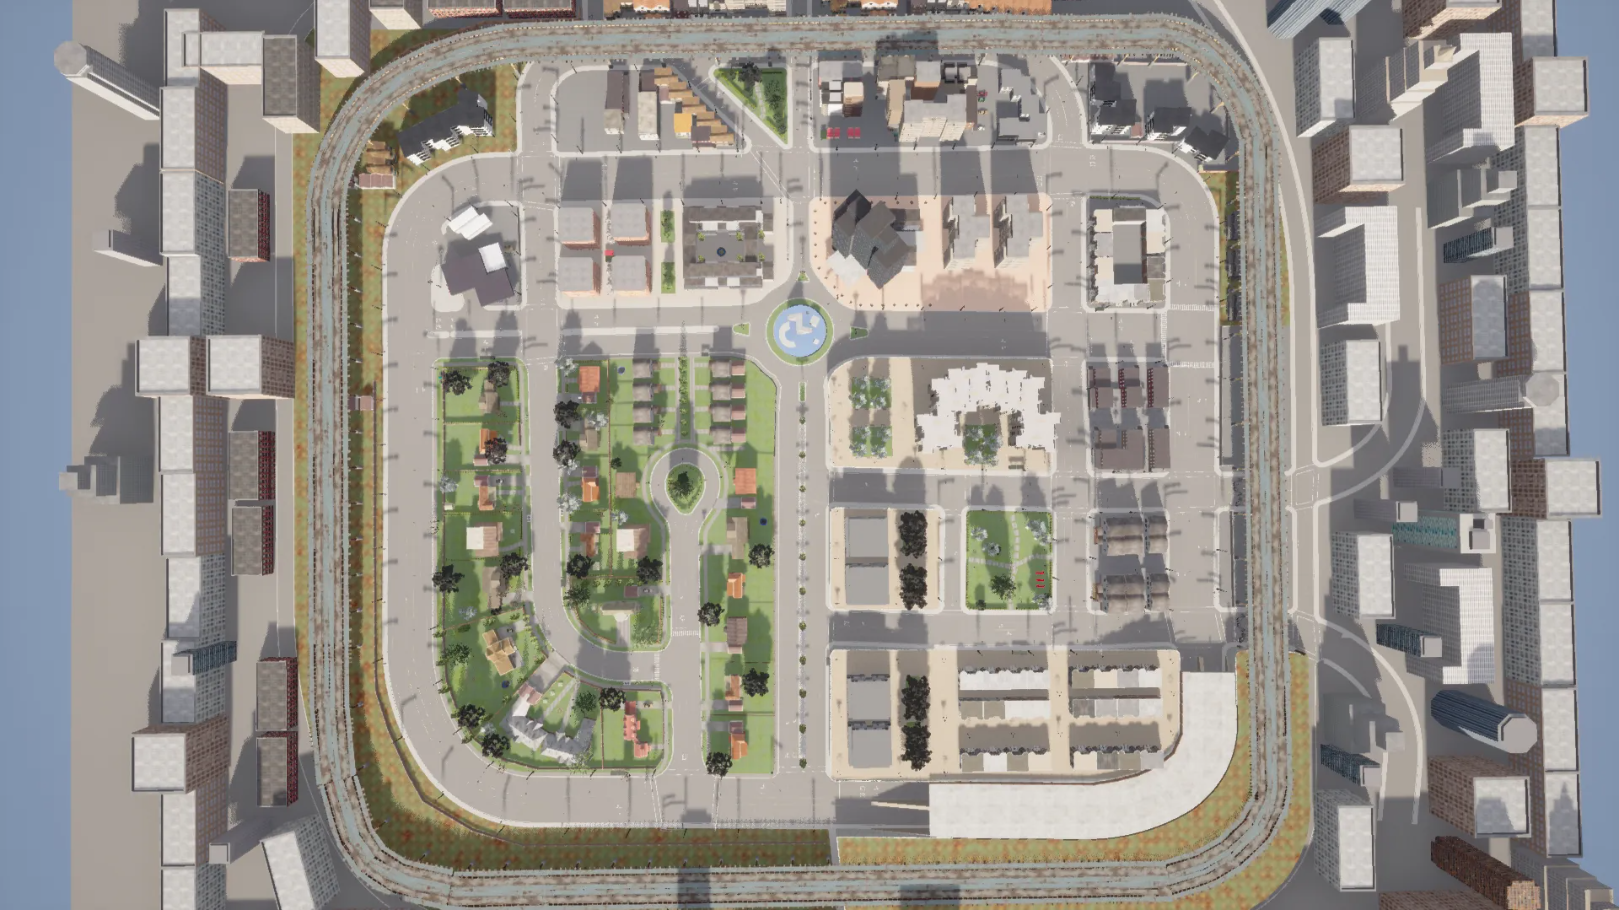
\includegraphics[width=\linewidth]{img/carla/town03.png}
        \caption{CARLA Town03 layout}
    \end{subfigure}
    \hfill
    \begin{subfigure}{0.48\textwidth}
        \centering
        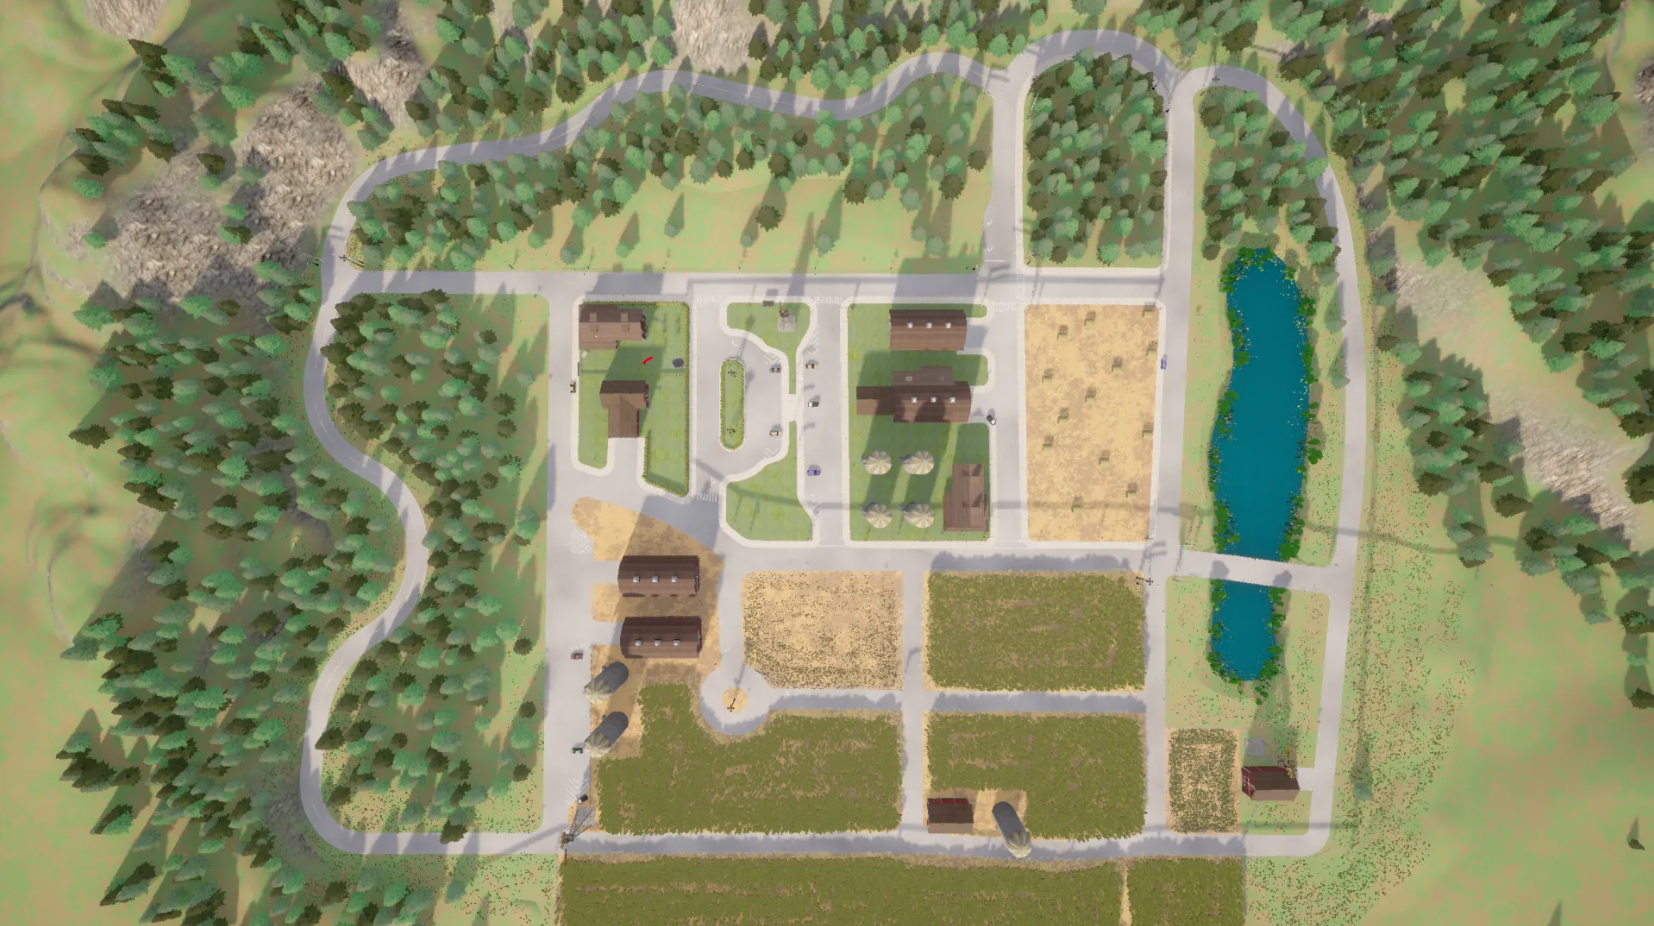
\includegraphics[width=\linewidth]{img/carla/town_7.png}
        \caption{CARLA Town07 layout}
    \end{subfigure}
    \caption{Top-down map layouts of the selected CARLA towns used for dataset collection~\cite{CARLA2024}}.
    \label{fig:carla_maps}
\end{figure}

\begin{figure}[htbp]
    \centering
    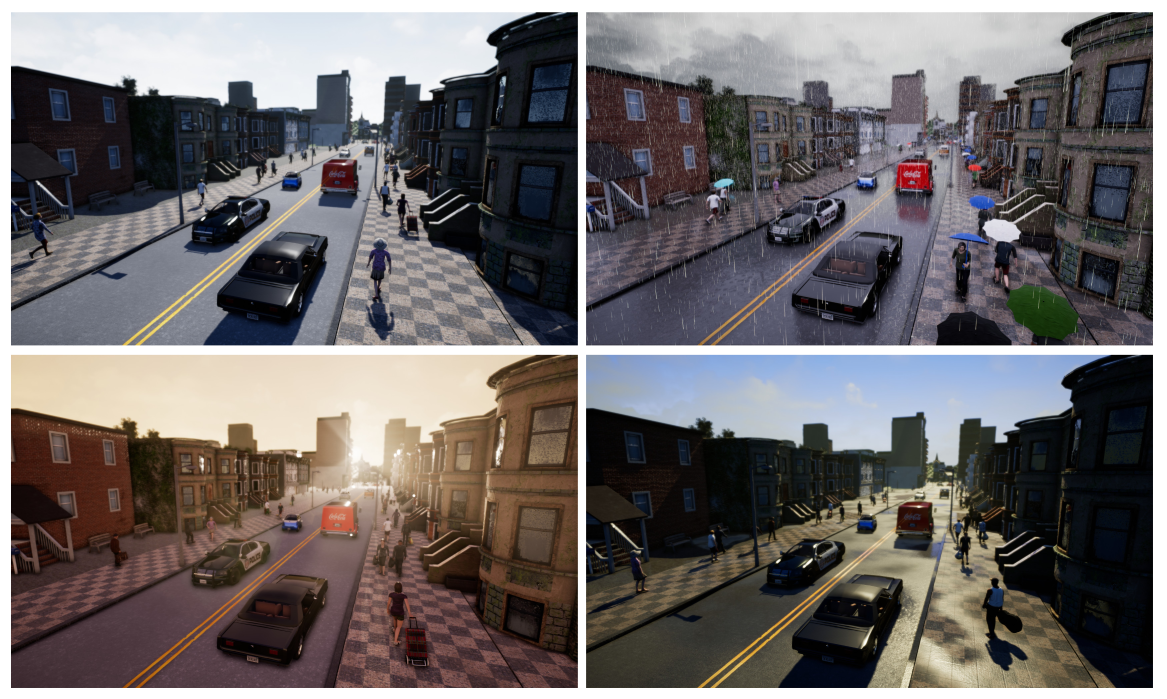
\includegraphics[width=0.7\linewidth]{img/carla/CARLA_Environment.png}
    \caption{3D Sample scenes from CARLA showcasing diverse conditions during dataset collection. The images illustrate a variety of urban and rural settings, with diverse lighting and weather conditions, including sunny, foggy, rainy, and snowy scenarios. Each scene highlights the flexibility of CARLA in simulating realistic driving environments for autonomous vehicle testing.}
    \label{fig:carla_scenes}
\end{figure}


Before executing any client-side scripts for dataset collection, it is essential to start the CARLA server using the following command in the CARLA root directory: ./CarlaUE4.sh


This launches the CARLA simulation in the Unreal Engine environment. For smooth operation, it is recommended to run the project on a system with at least \textbf{16 GB of RAM}, a dedicated GPU (e.g., \textbf{NVIDIA RTX series}), and \textbf{Ubuntu 18.04 or 20.04 LTS}. 

For the development and training of the Variational Autoencoder (VAE) and classifier models, we used \textbf{Python version 3.11 or higher}. This was necessary to avoid compatibility issues with newer versions of PyTorch, which are not well supported on older Python versions like 3.7. While dataset collection was handled using Python 3.7, the core machine learning model development required a more modern Python environment.  

To monitor and interpret various aspects of model training such as loss, accuracy, weight distributions, and layer activations we used \textbf{TensorBoard}. It provided valuable insights into training behavior and helped fine-tune model performance.

\section{Dataset Collection, Labeling, and Splitting Process}

To train and evaluate the proposed models effectively, a high-quality and well-structured dataset was essential. A systematic data preparation pipeline consisting of three key stages \textit{collection}, \textit{labeling}, and \textit{splitting}. The dataset was first collected using the CARLA simulator, which offers a controllable and realistic environment for simulating diverse driving scenarios. Following data collection, a precise rule-based labeling strategy was applied using vehicle control signals to assign meaningful class labels. Finally, the labeled dataset was partitioned into training and testing subsets to ensure class balance and prevent data leakage. This structured pipeline ensured consistency, and reproducibility  throughout the experimental workflow.

\subsection{Dataset Collection}

The dataset was collected using the CARLA simulator~\cite{CARLA2024docs}. An Audi A2 vehicle was deployed in autopilot mode to autonomously navigate the environment while capturing RGB images and corresponding control signals. A front mounted RGB camera was configured with a 125° field of view (FoV) and a resolution of $160 \times 80$ pixels. This resolution was selected to balance computational efficiency with sufficient visual detail for model learning.

A total of approximately 12,000 images were collected under varied driving scenarios. Each image was paired with the vehicle’s control parameters steering, throttle, and brake. The \textit{steering angle} ranged from $-1$ (full left) to $1$ (full right), while \textit{throttle} and \textit{brake} values ranged from $0$ to $1$, representing the intensity of acceleration and braking, respectively. This multi-modal data captured both visual context and driving behavior. The resulting dataset served as the foundation for both binary (STOP vs. GO) and multi-class (STOP, GO, LEFT, RIGHT) classification tasks.


\subsection{Dataset Labeling}

The collected data was labeled using a deterministic rule-based strategy derived from the vehicle’s control inputs. Two distinct labeling schemes were implemented to support binary and multi-class classification objectives.

For the \textbf{binary-class scheme}, each frame was labeled as either \texttt{STOP} or \texttt{GO}. A frame was labeled as \texttt{STOP} if the brake value exceeded a predefined threshold. Otherwise, it was labeled as \texttt{GO}. This distinction effectively captured the vehicle's motion state based on braking behavior.

For the \textbf{multi-class scheme}, labels were assigned based on prioritized control logic:
\begin{itemize}
    \item STOP, if the brake value exceeded a defined threshold.
    \item RIGHT, if the steering value was significantly positive and throttle was active.
    \item LEFT, if the steering value was significantly negative and throttle was active.
    \item GO, for all remaining cases where the vehicle moved straight without braking or significant steering.
\end{itemize}

This approach ensured mutually exclusive and semantically meaningful labels for each image. Threshold values for labeling were empirically determined based on the distribution of control signals across the dataset. The process was fully automated, ensuring reproducibility and eliminating manual labeling bias.

\subsection{Dataset Splitting}

Following labeling, the dataset was divided into separate training and testing subsets. The splitting was performed \textit{after} labeling to maintain label integrity and avoid any form of data leakage. Care was taken to ensure that the distribution of class labels remained balanced across both sets. This was critical for promoting fair learning and evaluation, particularly in the multi-class scenario.

The labeled dataset was partitioned using an 80/20 split ratio, where 80\% of the data was used for training and 20\% for testing. This ensured sufficient data for model learning while preserving a representative set for evaluation.

For the binary classification scheme, the training set contained 4,959 GO and 4,728 STOP samples, while the test set included 1,262 GO and 1,160 STOP samples, maintaining a near-balanced distribution across classes. Similarly, for the 4-class setting, all classes (GO, STOP, LEFT, RIGHT) were equally represented with 3,327 samples in training and 821 samples per class in testing. The distributions for both schemes are visualized side by side in Figure~\ref{fig:label_distribution_combined}.


\begin{figure}[htbp]
    \centering
    \begin{subfigure}{0.48\textwidth}
        \centering
        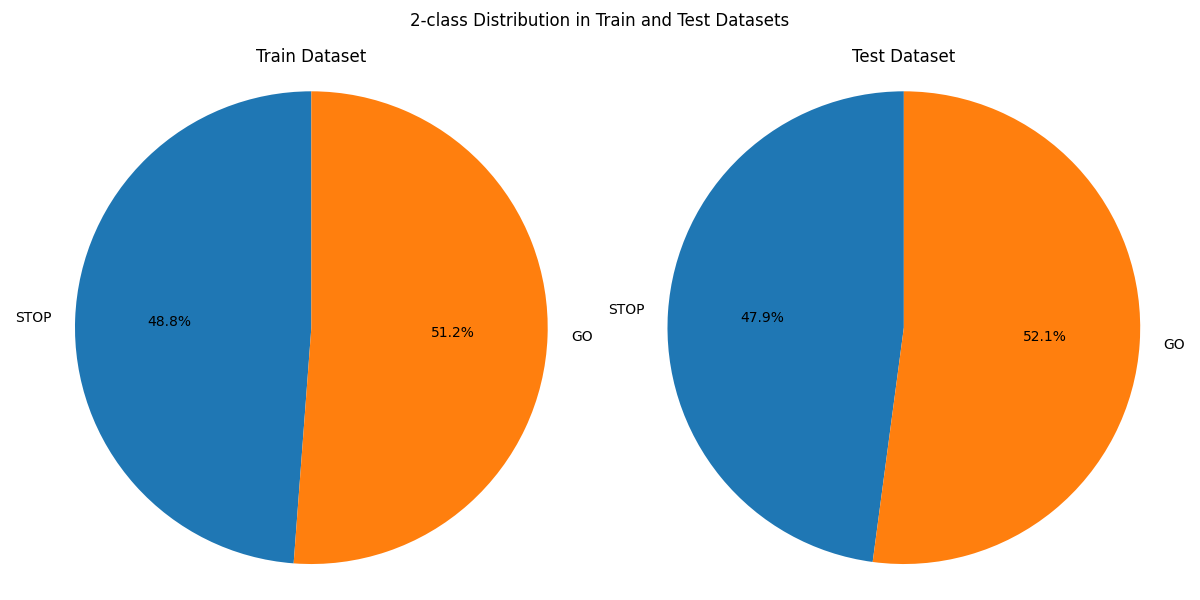
\includegraphics[width=\linewidth]{img/dataset/2class_distribution.png}
        \caption{Binary class (GO, STOP) label distribution}
        \label{fig:binary_class_distribution}
    \end{subfigure}
    \hfill
    \begin{subfigure}{0.5\textwidth}
        \centering
        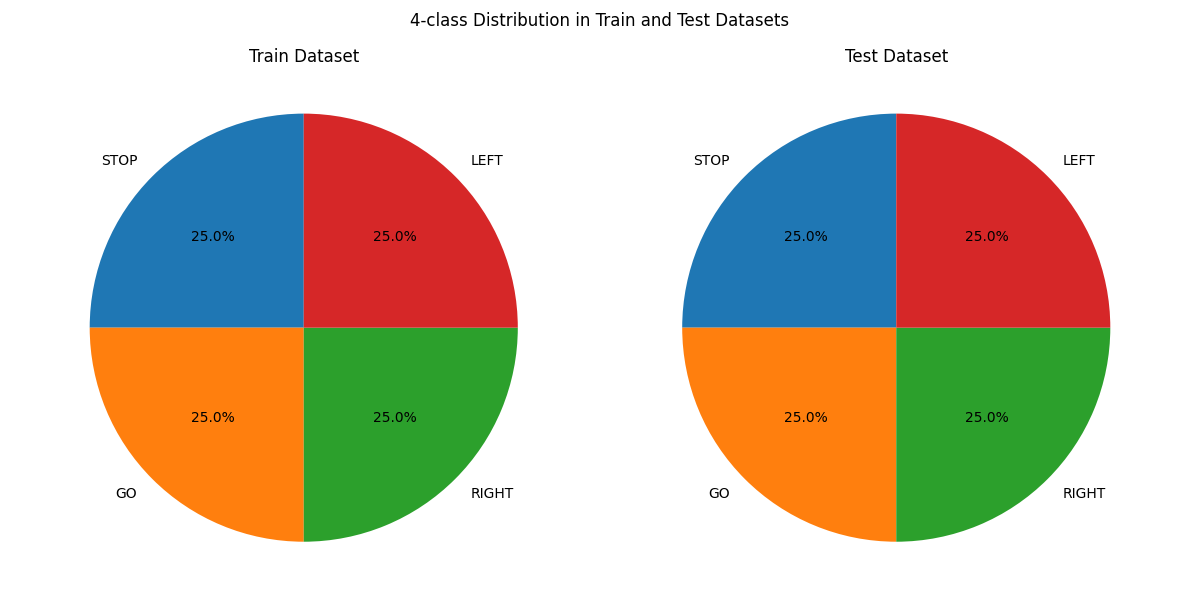
\includegraphics[width=\linewidth]{img/dataset/4class_distribution.png}
        \caption{multi-class label distribution (GO, STOP, LEFT, RIGHT)}
        \label{fig:class_distribution_pie}
    \end{subfigure}
    \caption{Label distributions across training and testing datasets for binary and multi-class classification schemes.}
    \label{fig:label_distribution_combined}
\end{figure}





\section{Variational Autoencoder (VAE)} \label{sec:vae}

This section outlines the architectural design, training process for the Variational Autoencoder (VAE) used in this work which strongly answers RQ1. The VAE serves as a generative backbone for producing realistic and plausible counterfactual explanations in the context of autonomous driving. Each component of the system is described in detail, along with the rationale for the chosen configurations and metrics.

To generate semantically coherent and visually realistic counterfactual explanations that remain on the data manifold, we adopt a Variational Autoencoder (VAE) as the generative backbone of our system. This approach draws conceptual motivation from the Contrastive Explanation Method (CEM)~\cite{DBLP:journals/corr/abs-1802-07623}, which leverages autoencoders to constrain generated samples within the support of the data distribution. While CEM was originally evaluated on low-dimensional datasets such as MNIST, our application domain involves high-resolution RGB images from complex driving scenarios. Consequently, the VAE architecture, training objective, and optimization strategy were carefully adapted and refined over multiple design iterations.

\subsection{VAE Architecture} \label{sec:vae_architecture}

The VAE consists of two primary components, a convolutional encoder that transforms the input image into a latent distribution, and a decoder that reconstructs the image from a sampled latent vector. The encoder and decoder are trained jointly using a variational loss function that enforces both reconstruction fidelity and latent space regularization.

\subsubsection{Encoder Architecture} \label{subsubsec:vae_encoder}

The encoder takes an input image of shape $3 \times 80 \times 160$ (RGB, height $\times$ width) and compresses it into a 128-dimensional latent space. The architecture is composed of four convolutional blocks followed by fully connected layers:

\begin{itemize}
    \item \textbf{Conv Layer 1:} 64 filters, kernel size $4 \times 4$, stride 2, no padding. Followed by LeakyReLU.
    \item \textbf{Conv Layer 2:} 128 filters, kernel size $3 \times 3$, stride 2, padding 1. Followed by BatchNorm and LeakyReLU.
    \item \textbf{Conv Layer 3:} 256 filters, kernel size $4 \times 4$, stride 2. Followed by LeakyReLU.
    \item \textbf{Conv Layer 4:} 512 filters, kernel size $3 \times 3$, stride 2. Followed by BatchNorm and LeakyReLU.
\end{itemize}

The final feature map output is flattened and passed through a fully connected layer with 1024 units (with LeakyReLU activation). From this, two separate linear layers output the mean vector $\mu \in \mathbb{R}^{128}$ and log-variance vector $\log\sigma^2 \in \mathbb{R}^{128}$, representing the parameters of the approximate posterior $q(z|x)$.

\subsubsection{Latent Sampling via Reparameterization Trick}
The latent vector $z$ is sampled using the reparameterization trick:
\begin{equation}
z = \mu + \sigma \cdot \epsilon, \quad \epsilon \sim \mathcal{N}(0, I)
\end{equation}
This allows gradient-based optimization through the stochastic sampling process, maintaining end-to-end differentiability. The encoder uses PyTorch’s native implementation of a normal distribution to sample $\epsilon$, and places the distribution tensors on the correct device (CPU or GPU).




\subsubsection{Decoder Architecture} \label{subsubsec:vae_decoder}

The decoder reverses the encoding process and reconstructs an image from the latent vector $z \in \mathbb{R}^{128}$. It consists of two fully connected layers followed by four transposed convolutional layers:

\begin{itemize}
    \item \textbf{Dense Layer 1:} Linear projection from 128 to 1024 units with LeakyReLU.
    \item \textbf{Dense Layer 2:} Linear projection from 1024 to $512 \times 4 \times 9 = 18432$ units, reshaped to $(512, 4, 9)$.
\end{itemize}

The reshaped feature map is then passed through:

\begin{itemize}
    \item \textbf{Deconv Layer 1:} 256 filters, kernel size $4 \times 4$, stride 2, padding 1, output padding (0,1). Followed by LeakyReLU.
    \item \textbf{Deconv Layer 2:} 128 filters, kernel size $4 \times 4$, stride 2, padding 1, output padding (1,1). Followed by LeakyReLU.
    \item \textbf{Deconv Layer 3:} 64 filters, kernel size $4 \times 4$, stride 2. Followed by LeakyReLU.
    \item \textbf{Deconv Layer 4:} 3 filters (RGB), kernel size $4 \times 4$, stride 2. Followed by Sigmoid activation.
\end{itemize}

The final output has shape $3 \times 80 \times 160$, matching the input dimensions. The Sigmoid activation ensures output values lie in the normalized $[0,1]$ range.


\subsection{Image Preprocessing and Augmentation Strategy} \label{subsec:vae_preprocessing}

To improve the generalization ability of the VAE and ensure robustness during training, a set of preprocessing and data augmentation techniques were applied. These techniques were chosen to address common challenges in real-world visual data such as occlusion, viewpoint variation, and overfitting.


During training, the following transformations were applied:
\begin{itemize}
    \item \textbf{Image Resizing:} All images were resized to a fixed resolution of $80 \times 160$ pixels to match the input dimensions required by the encoder.
    \item \textbf{Random Horizontal Flip:} Each image was horizontally flipped with a 50\% probability to simulate mirrored driving conditions and improve generalization.
    % \item \textbf{Random Masking:} A random rectangular region covering 10\% of the image area was masked (set to zero). This augmentation was not only intended to encourage the model to learn robust feature representations by reconstructing occluded regions, but also to strategically expose the VAE to incomplete visual inputs during training. The primary motivation was to ensure that the model remains effective when applied in later stages of this thesis, particularly in masking-based counterfactual generation—where masked or altered inputs are a core component of the explanation process. Training the VAE under such conditions improves its ability to reconstruct high-fidelity outputs even when parts of the input are missing or corrupted.
    \item \textbf{Tensor Conversion:} Images were converted to PyTorch tensors and scaled from [0, 255] to [0.0, 1.0] before being passed to the network.
\end{itemize}


For the testing phase, only the essential deterministic transformations were applied:
\begin{itemize}
    \item Image resizing to $80 \times 160$ pixels
    \item Tensor conversion with pixel scaling
\end{itemize}


\subsection{Training Objective and Optimization Strategy} \label{subsec:vae_loss}

This section presents the training objective and optimization strategy employed to train the Variational Autoencoder (VAE). Including these details in the methodology is essential not only for ensuring reproducibility but also for highlighting the specific design choices that enabled the VAE to learn robust latent representations—central to generating counterfactual explanations in subsequent stages of this work.

The VAE is trained using a composite variational loss function, defined as:
\[
\mathcal{L}_{\text{VAE}} = \mathcal{L}_{\text{recon}} + \lambda_{\text{KL}} \cdot \mathcal{L}_{\text{KL}}
\]
where $\mathcal{L}_{\text{recon}}$ denotes the reconstruction loss, and $\mathcal{L}_{\text{KL}}$ represents the Kullback-Leibler (KL) divergence. The scalar $\lambda_{\text{KL}}$ controls the regularization strength applied to the latent space.

\paragraph{Reconstruction Loss:} \label{reconstruction_loss}

To assess the impact of different loss formulations on reconstruction quality, two reconstruction loss functions were implemented and compared:
\begin{itemize}
    \item \textbf{Mean Squared Error (MSE):} Measures the average squared difference between corresponding pixel intensities of the input and reconstructed images. It emphasizes pixel-level fidelity and is a standard choice in image reconstruction tasks.
    \item \textbf{Log-Cosh Loss:} A smooth approximation of the Mean Absolute Error (MAE), which behaves like MSE for small differences and like MAE for large ones. It is more tolerant to outliers and encourages sharper reconstructions.
\end{itemize}

Empirical results showed that Log-Cosh yielded smoother and more visually coherent reconstructions during early training epochs, particularly in complex scenes. This finding is supported by prior work, such as Chen et al.~\cite{chen2019log}, and a detailed comparison is presented in \cref{subsec:vae_quant_comparison}.

\paragraph{KL Divergence Regularization:}

The KL divergence term ensures that the learned posterior distribution $q(z|x)$ remains close to the unit Gaussian prior $p(z) = \mathcal{N}(0, I)$:
\[
\mathcal{L}_{\text{KL}} = -\frac{1}{2} \sum_{i=1}^{d} \left(1 + \log\sigma_i^2 - \mu_i^2 - \sigma_i^2\right)
\]
This regularization helps enforce a well-structured latent space, enabling smooth interpolation and meaningful sampling—both of which are critical for generating plausible counterfactual samples.

\paragraph{KL Weight Annealing:}

To prevent the KL term from dominating the loss function too early in training before the reconstruction objective is sufficiently optimized a linear annealing strategy was used:
\[
\lambda_{\text{KL}} = \min(\lambda_0 + \delta \cdot \text{epoch}, 1.0)
\]
where $\lambda_0 = 5 \times 10^{-5}$ and $\delta = 1 \times 10^{-4}$. This allows the model to initially focus on accurate reconstruction and gradually introduce regularization, leading to a better trade-off between fidelity and latent structure.

\paragraph{Training Configuration:}

The VAE was implemented in PyTorch and trained on a Linux-based system using Python 3.11. Computation was accelerated via an NVIDIA CUDA-enabled GPU (e.g., RTX 1080 Ti). The following hyperparameters and strategies were adopted:

\begin{itemize}
    \item \textbf{Optimizer:} Adam, selected for its adaptive learning rate and momentum properties, which are particularly effective for optimizing non-convex objectives like those in VAEs.
    \item \textbf{Learning Rate:} $1 \times 10^{-4}$ — empirically chosen to ensure stable gradient updates and smooth convergence.
    \item \textbf{Weight Decay:} $1 \times 10^{-5}$ — applied as L2 regularization to prevent overfitting by penalizing large parameter magnitudes.
    \item \textbf{Batch Size:} 128 — balances GPU memory utilization and the statistical reliability of mini-batch gradients.
    \item \textbf{Epochs:} 200 — provides sufficient time for convergence, with early stopping to prevent overfitting.
    \item \textbf{Learning Rate Scheduler:} \texttt{ReduceLROnPlateau}, with patience = 10 and factor = 0.5 — dynamically reduces the learning rate when validation loss stagnates, enabling finer convergence.
    \item \textbf{Early Stopping:} Applied with a patience of 50 epochs — halts training when no validation improvement is observed, conserving computational resources.
\end{itemize}

This configuration was iteratively tuned to ensure the VAE could effectively learn semantically meaningful latent codes while remaining computationally efficient. The combination of a reliable optimizer (Adam), adaptive learning rate scheduling, loss annealing, and early stopping fosters a stable training regime. Each design decision contributes to the ultimate goal of generating high-quality, realistic counterfactual explanations that remain faithful to the original data distribution.

To monitor training progress, each epoch logged Total loss, Reconstruction loss, KL divergence, SSIM, and PSNR. These evaluations confirm the VAE's capacity to learn expressive, structured representations. The empirical performance of this architecture is presented and discussed in \cref{sec:vae_evaluation}, where its reconstruction fidelity, and latent space utility effectiveness are quantitatively and qualitatively evaluated.



\section{Classifier Architectures and Training Setup}
\label{sec:classifier_architectures}


To assess the semantic structure of the learned latent space and evaluate downstream task performance, multiple classifiers were trained using the 128-dimensional latent representations generated by the VAE encoder. Each image corresponds to a driving situation (e.g., STOP, GO, RIGHT, LEFT), and the classifiers were trained to predict the appropriate driving action class from the latent vector.

Unlike conventional approaches where classifiers are trained directly on pixel-level image data, this work emphasizes feature-based classification, operating solely in the compressed and semantically meaningful latent space. This allows for efficient model training, improved interpretability, and compatibility with counterfactual explanation techniques explored later in the thesis.

This section describes the architecture, training configurations, and optimization strategies used for each classifier. All models were trained and evaluated using the latent feature vectors extracted from the VAE encoder. The input to each classifier is a 128-dimensional feature vectors.

\subsection{Neural Network Classifier Training (MLP)} \label{subsec:neural_network_classifier_training}

A deep feedforward neural network was implemented using PyTorch to classify the latent vectors extracted from the VAE. The architecture was designed with simplicity and effectiveness in mind, specifically tailored to the 128-dimensional latent representations. This classifier is composed of three fully connected (dense) layers, each followed by batch normalization and dropout regularization, with LeakyReLU activations throughout. The details are as follows:

\begin{itemize}
    \item \textbf{Input size:} 128 \\
    The input to the network is a 128-dimensional vector, corresponding to the latent features produced by the VAE encoder. This compact representation captures the essential semantic information from the original image.
    
    \item \textbf{Hidden layers:} 3 layers, each with 128 units \\
    Three fully connected hidden layers were chosen to provide the network with sufficient capacity to model non-linear relationships within the latent space. Maintaining a consistent layer size (128 units) aligns with the dimensionality of the latent vector, ensuring that each hidden layer can process the full feature set without dimensionality reduction, which helps preserve the rich information embedded in the latent space.
    
    \item \textbf{Activation:} LeakyReLU with slope 0.01 \\
    LeakyReLU is used as the activation function for its advantages over the traditional ReLU. Unlike ReLU, which zeroes out negative inputs, LeakyReLU allows a small, non-zero gradient (with a slope of 0.01) for negative values. This feature mitigates the "dying ReLU" problem, ensuring that neurons do not become inactive during training and thereby promoting better gradient flow across the network.
    
    \item \textbf{Regularization:} Dropout (p = 0.5) and Batch Normalization \\
    Dropout is applied with a probability of 0.5 after each hidden layer to prevent overfitting by randomly deactivating half of the neurons during training. This forces the network to learn more robust features that are not overly dependent on any single neuron. Batch Normalization is applied to stabilize and accelerate training by normalizing the inputs to each layer. It reduces internal covariate shift, which helps in achieving faster convergence and improved overall performance.
    
    \item \textbf{Output:} 2 or 4 logits depending on classification task \\
    The final output layer produces either 2 or 4 logits, corresponding to the binary or multi-class classification tasks, respectively. The logits represent the unnormalized scores for each class, and a softmax function is applied during loss computation (using CrossEntropy Loss) to obtain probability distributions over the classes.
\end{itemize}

This architecture was selected because it effectively balances model complexity and computational efficiency, making it well-suited for the compact and informative VAE latent space. By leveraging non-linear activations and regularization techniques, the network is capable of learning subtle distinctions between classes while mitigating overfitting, ultimately yielding strong classification performance. The evaluation and performance comparison of this classifier, along with other traditional models trained on latent features, are discussed in Section~\ref{sec:classifier_eval}.




\subsection{Traditional Classifiers}
\label{subsec:traditional_classifiers}

To compare the neural classifier's performance with classical machine learning models, the following classifiers were implemented using the scikit-learn library~\cite{scikit-learn}. All models were trained on 128-dimensional latent vectors extracted from the VAE encoder. The dataset was split in an 80:20 ratio for training and testing. Each model was evaluated using precision, recall, F1-score, accuracy, confusion matrix, and ROC-AUC metrics (see \cref{subsec:comparision_with_traditional_classifiers}).

\subsubsection{Logistic Regression: Implementation and Training}
\label{subsubsec:logistic_regression}
Logistic Regression was implemented as a linear baseline model using scikit-learn’s \textit{LogisticRegression}~\cite{scikit-learn} with one-vs-rest (OvR) strategy and L2 regularization. This model was used to assess how linearly separable the VAE-generated latent space is. In the multi-class configuration, the OvR strategy enabled independent binary classifiers for each class.

\subsubsection{K-Nearest Neighbors (KNN): Implementation and Training}
\label{subsubsec:knn}
The K-Nearest Neighbors (KNN) classifier was implemented using scikit-learn’s \textit{KNeighborsClassifier}~\cite{Cover1967} with $k=5$, employing Euclidean distance to compute nearest neighbors. KNN was used to explore how local neighborhood structure manifests in the latent feature space. As an instance-based model, it does not require explicit training and makes predictions based on majority voting among the $k$ nearest training samples.

\subsubsection{Random Forest: Implementation and Training}
\label{subsubsec:random_forest}
Random Forest was implemented as an ensemble of 100 decision trees using scikit-learn’s \textit{RandomForestClassifier}~\cite{Breiman2001}. The model was trained with default settings, letting the maximum tree depth be inferred automatically. This ensemble-based approach allowed the model to evaluate complex decision boundaries and learn from diverse latent patterns in the data.

\subsubsection{Support Vector Machine (SVM): Implementation and Training}
\label{subsubsec:svm}
Support Vector Machine (SVM)~\cite{Cortes1995} was implemented using scikit-learn’s \textit{SVC} with a radial basis function (RBF) kernel and probability estimates enabled. The RBF kernel allows the model to project latent features into a higher-dimensional space, which is helpful for modeling non-linear boundaries. This configuration was used to assess the effectiveness of margin-based classification in the VAE latent space.




\section{Feature Masking Techniques for Finding Counterfactual Explanations}
\label{sec:feature_masking_pipeline}

To generate counterfactual explanations (CEs), multiple feature masking strategies were employed. These strategies differ in terms of their perturbation space (image space or latent space) and masking mechanism, but all aim to identify minimal changes in the input that alter the classifier’s decision.

All methods follow a unified processing pipeline comprising the following steps:

\begin{enumerate}
    \item Encode the original image using the encoder of a Variational Autoencoder (VAE) to obtain a latent representation.
    \item Classify the latent vector using a trained classifier to obtain the original prediction.
    \item Apply a masking strategy (in image space or latent space).
    \item Reconstruct the masked or modified input using the decoder.
    \item Re-encode the reconstructed image and classify the new latent vector.
    \item Compare the new prediction with the original. If different, the result is identified as a counterfactual explanation.
\end{enumerate}

While the decoding and re-encoding steps (Steps 4 and 5) may seem like extra effort, they play a crucial role in ensuring the quality and reliability of the generated counterfactuals. After masking certain latent features in Step 3, the modified vector may no longer represent a meaningful or valid sample. If we were to directly classify this altered latent vector, there’s a good chance the prediction would be unstable or even nonsensical. This is because the classifier has only seen latent vectors produced by the encoder during training not arbitrary, masked ones.

To address this, the masked latent vector is first passed through the decoder to generate an image (Step 4). This step effectively "fills in the blanks" using the decoder’s understanding of the dataset. It acts like an inpainting mechanism that ensures the resulting image still looks realistic and semantically coherent. Then, instead of classifying this image directly, it is passed through the encoder once again (Step 5). This gives us a latent vector that the classifier can safely work with, as it now comes from the same distribution it was trained on.

This extra step of decoding and re-encoding serves two important purposes. First, it keeps the modified input within the data manifold, ensuring that we're generating plausible counterfactuals rather than random noise. Second, it helps maintain the integrity of the classification process, ensuring that the classifier is not thrown off by unfamiliar or unnatural inputs.

It also has an additional benefit: it allows us to visualize the counterfactual in the form of an actual image. This is especially useful in image-based domains like autonomous driving, where interpretability is just as important as accuracy. Seeing the visual differences between the original and counterfactual inputs helps us understand what specific features influenced the model’s decision.


Furthermore, the masking techniques used in this work are broadly divided into two categories based on where the perturbation is applied: (1) masking in the image space, and (2) masking in the latent space. Each of these is discussed in detail in the following subsections.

\subsection*{Image Space Masking}
This includes Grid-Based Masking, LIME on Images, and Object Detection-Based Masking. These methods apply masking directly to the input image.
\begin{itemize}
    \item \textbf{Grid-Based Masking:} The image is divided into grids (e.g., 10$\times$5, 4$\times$2), and each cell is masked iteratively to observe prediction changes.
    \item \textbf{LIME on Images:} LIME is applied on pixel space to identify important regions, which are then masked.
    \item \textbf{Object Detection-Based Masking:} YOLOv5 is used to detect semantic objects (e.g., pedestrians, vehicles), which are then removed from the image by zeroing out pixels in the bounding box.
\end{itemize}

\subsection*{Latent Space Masking}
This includes LIME on Latent Features and LIME with nearest-unlike-neighbour (NUN). Here, perturbations are applied to the encoded latent vector.
\begin{itemize}
    \item \textbf{LIME on Latent Features:} LIME identifies influential latent dimensions. These are replaced using strategies such as median substitution or rule-based adjustments using dataset statistics.
    \item \textbf{LIME-Guided Latent Feature Masking using NUN:} Combines LIME-based feature importance with the nearest-unlike-neighbour strategy, selecting feature replacements that are more robust and semantically meaningful. LIME-Guided Latent Feature Masking using NUN is formally called LIME with NUN throughout the thesis.
\end{itemize}

For each method, similarity metrics (SSIM, PSNR, MSE, UQI, VIFP) are computed between the original and reconstructed images to assess visual fidelity. All results, including prediction changes, classifier confidences, masking parameters, and processing time, are logged into method-specific files for analysis. If the prediction changes after masking, the example is labeled as a successful counterfactual. This analysis directly supports answering the research question outlined in \cref{sec:research_question}, particularly \textbf{RQ3}.


In the subsequent subsections, each masking method is detailed along with its algorithm, implementation logic.
 

\subsection{Grid-Based Masking} \label{sec:grid_based_masking}

Grid-based masking is a spatial perturbation technique designed to generate counterfactual explanations (CEs) by selectively occluding small square regions of an input image. The underlying assumption is that certain spatial regions exert a disproportionate influence on the model’s classification decision. By masking these regions and observing changes in the model’s output, we can gain insights into which parts of the input image are causally relevant for the decision-making process.

This method follows the general feature masking pipeline outlined in Section~\ref{sec:feature_masking_pipeline}. First, the input image is encoded into a latent representation using a Variational Autoencoder (VAE). The latent features are passed to a classifier to generate the original prediction, and the image is also reconstructed via decoding for consistency. The masking operation is applied directly to the pixel space by zeroing out specific spatial regions (grid cells) before the image is re-encoded, reconstructed, and re-evaluated by the classifier.

To balance localization precision and computational efficiency, we experimented with multiple grid sizes and empirically selected two square grid configurations based on performance. 

\begin{itemize}
    \item \textbf{Fine grid:} $8 \times 16$ (each cell is $10 \times 10$ pixels)
    \item \textbf{Coarse grid:} $4 \times 8$ (each cell is $20 \times 20$ pixels)
\end{itemize}

These configurations were chosen in alignment with the image resolution ($160 \times 80$), ensuring uniform spatial coverage without distorting the image’s structure. The fine grid enables detailed localization of influential features, while the coarse grid offers broader contextual masking. During preliminary experiments, alternative grid sizes such as $10 \times 5$ and $4 \times 2$ were also evaluated. However, the square-like configurations were found to yield more reliable and interpretable results, likely due to their equal-area masking and reduced spatial bias.

\begin{figure}[htbp]
\centering
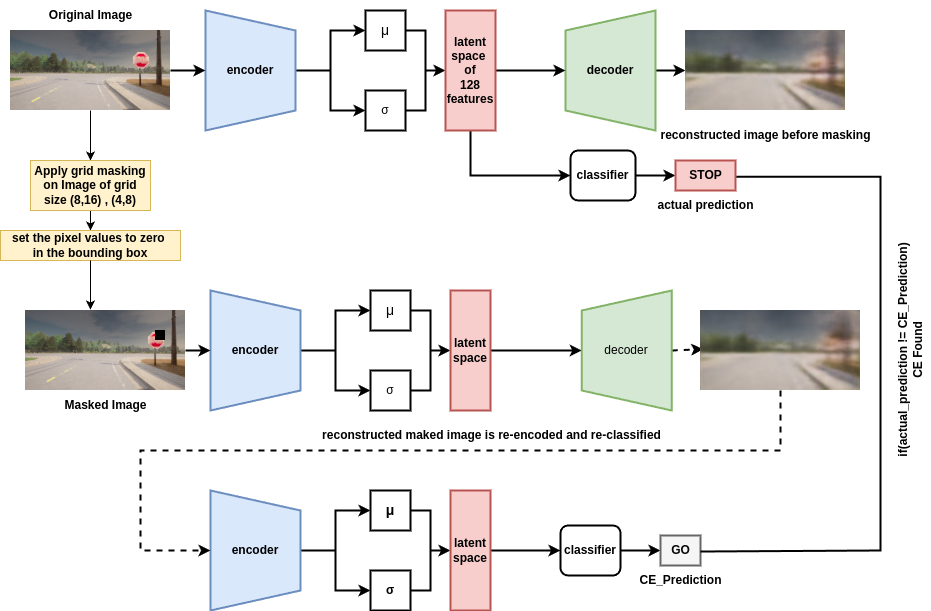
\includegraphics[width=0.95\textwidth]{img/masking/grid_based_masking/grid_based_masking_flow.drawio.png}
\caption{Workflow of the grid-based counterfactual generation process. Grid cells are masked sequentially in two stages: a fine grid ($8 \times 16$) and a coarse grid ($4 \times 8$). Masked images are reconstructed using a VAE and re-evaluated by the classifier. A prediction change implies that the masked region was causally important.}
\label{fig:grid_masking_diagram}
\end{figure}

The masking follows a sequential strategy, beginning with the finer grid. Each cell is masked individually by zeroing its pixel values. If masking any one cell results in a change in the model’s prediction, a counterfactual is deemed to have been found, and the process terminates early. This behavior adheres to the principle of \textit{minimal intervention}~\cite{wachter2018CE}, wherein the smallest possible change is sufficient to alter the decision. If no counterfactual is detected in the fine grid, the search continues with the coarse grid.

Once a cell is masked, the resulting image is passed through the encoder-decoder pipeline to maintain visual plausibility. The reconstructed image is then re-encoded and classified. A prediction change signifies that the masked region played a decisive role in the original decision, and thus constitutes a valid counterfactual explanation.


\vspace{1em}
\begin{algorithm}[htbp]
\caption{Grid-Based Masking for Counterfactual Generation}
\label{alg:grid_based_masking}
\begin{algorithmic}[1]
\REQUIRE Image $I$, encoder $E$, decoder $D$, classifier $C$, grid configurations $G = \{(8,16), (4,8)\}$
\ENSURE Whether a counterfactual explanation is found

\STATE Encode image: $z \leftarrow E(I)$
\STATE Predict original label: $y_{\text{orig}} \leftarrow \arg\max C(z)$

\FOR{each grid size $(m, n)$ in $G$}
    \STATE $T \leftarrow m \times n$
    \FOR{$p = 0$ to $T - 1$}
        \STATE Mask grid cell $p$ in $I$ to obtain $I_{\text{masked}}$
        \STATE Encode: $z_{\text{masked}} \leftarrow E(I_{\text{masked}})$
        \STATE Decode: $I_{\text{recon}} \leftarrow D(z_{\text{masked}})$
        \STATE Re-encode: $z_{\text{re}} \leftarrow E(I_{\text{recon}})$
        \STATE Predict: $y_{\text{new}} \leftarrow \arg\max C(z_{\text{re}})$
        \IF{$y_{\text{new}} \neq y_{\text{orig}}$}
            \RETURN Counterfactual explanation found
        \ENDIF
    \ENDFOR
\ENDFOR

\RETURN No counterfactual explanation found
\end{algorithmic}
\end{algorithm}
% \vspace{1em}


Figure~\ref{fig:grid_masking_diagram} illustrates the complete grid-based masking workflow. It highlights how the original image is masked, reconstructed, and re-classified. A prediction change from \texttt{STOP} to \texttt{GO} following the masking of a grid cell demonstrates the effectiveness of this approach in revealing causally salient regions. The masked region is processed through a VAE to maintain visual plausibility, ensuring that the model’s reaction is not triggered by implausible image artifacts.

\begin{figure}[htbp]
\centering
\begin{subfigure}[b]{0.3\textwidth}
    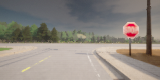
\includegraphics[width=\textwidth]{img/masking/grid_based_masking/original.png}
    \caption{Original Image}
    \label{fig:grid_orig}
\end{subfigure}
\hfill
\begin{subfigure}[b]{0.3\textwidth}
    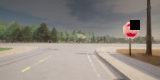
\includegraphics[width=\textwidth]{img/masking/grid_based_masking/reconstructed_grid_masked_image.png}
    \caption{Masked Grid Region}
    \label{fig:grid_masked}
\end{subfigure}
\hfill
\begin{subfigure}[b]{0.3\textwidth}
    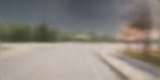
\includegraphics[width=\textwidth]{img/masking/grid_based_masking/CE_grid.png}
    \caption{Reconstructed CE Image}
    \label{fig:grid_recon}
\end{subfigure}
\caption{
Counterfactual explanation generated using grid-based masking. (a) The original image is classified as \texttt{STOP}. (b) A specific grid cell overlapping the STOP sign is masked (blackout). (c) The masked image is reconstructed using a VAE, and reclassified as \texttt{GO}. The change in prediction indicates that the masked region contained causally important features responsible for the initial decision. This result exemplifies the effectiveness of spatial masking in isolating minimal influential regions.
}
\label{fig:grid_ce_example}
\end{figure}

Figure~\ref{fig:grid_ce_example} illustrates the counterfactual generation process using the proposed grid-based masking method. A fine grid is applied to the original image, and each cell is evaluated sequentially. In this instance, masking a specific cell overlapping the STOP sign caused the classifier to change its prediction from \texttt{STOP} to \texttt{GO}. This confirms that the masked region was essential to the model’s decision. The reconstructed image, generated via a Variational Autoencoder, remains visually plausible, ensuring that the change in classification is not due to unrealistic input artifacts.




\subsection{Object Detection-Based Masking} \label{sec:object_detection_masking}

Object Detection-Based Masking introduces a semantically informed approach for generating counterfactual explanations by selectively removing identifiable real-world objects from complex driving scenes. The motivation behind this method is grounded in the causal interpretability of autonomous systems: understanding which specific entities—such as traffic signs, vehicles, pedestrians, or road infrastructure—directly influence a model's driving decision can provide actionable insights into the model's internal reasoning.

Following the general masking pipeline described in Section~\ref{sec:feature_masking_pipeline}, this approach utilizes a Variational Autoencoder (VAE) to encode the original input image into a latent space, which is then passed through a classifier to obtain the model’s initial prediction. However, rather than relying on low-level spatial patterns (as in grid-based masking), this method employs semantic object detection to guide the masking process.

To achieve this, a pre-trained YOLOv5 model~\cite{jocher2020yolov5} is integrated into the pipeline to detect and localize objects present in the input image. The full workflow is illustrated in Figure~\ref{fig:object_detection_workflow}, combining object detection, VAE-based reconstruction, and classifier re-evaluation to identify counterfactuals. YOLOv5 is a single-stage object detector known for its speed and accuracy across 80 COCO classes~\cite{lin2015microsoftcococommonobjects}, including vehicles, persons, and traffic control elements. Each detected object is described by a bounding box $(x_{\min}, y_{\min}, x_{\max}, y_{\max})$, which defines the region to be masked. The overall procedure is summarized in Algorithm~\ref{alg:object_detection_masking}.

\begin{figure}
    \centering
    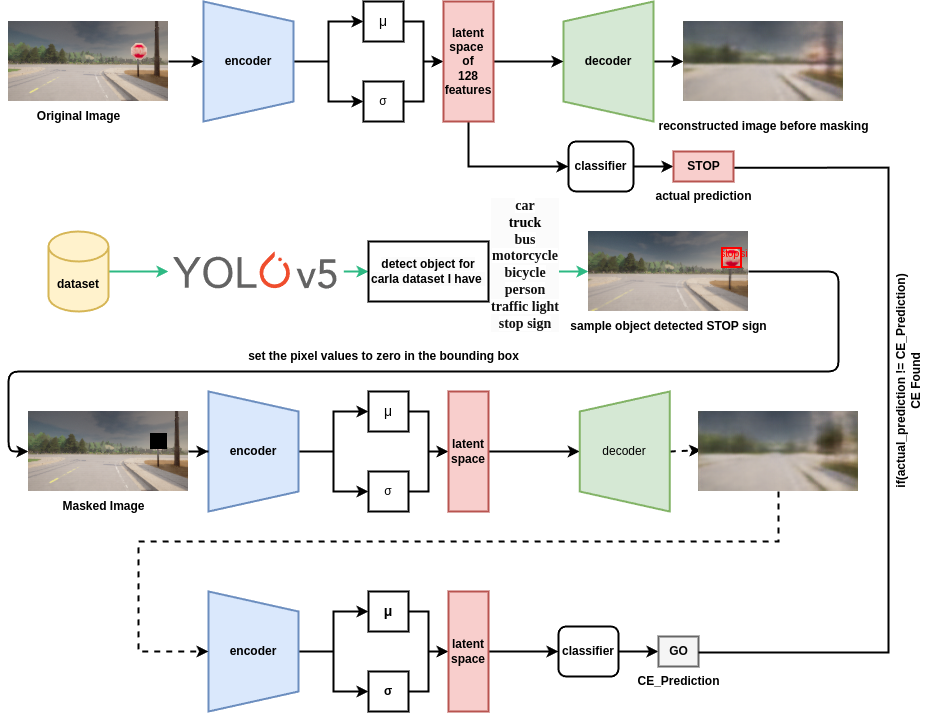
\includegraphics[width=0.95\textwidth]{img//masking//object_detection/object_detection_based_masking_flow.drawio.png}
    \caption{
Workflow of the object detection-based counterfactual explanation pipeline. The input image is first encoded using a Variational Autoencoder (VAE) to obtain a latent representation. The classifier predicts the original driving decision (e.g., \texttt{STOP}). Simultaneously, a pre-trained YOLOv5 detector identifies objects in the image. One detected object (e.g., a STOP sign) is masked and passed through the encoder-decoder pipeline to reconstruct a visually plausible image. If reclassification of this reconstruction results in a different label (e.g., \texttt{GO}), a counterfactual explanation is found. The process is iterated per object, and the first valid counterfactual is retained.
}
\label{fig:object_detection_workflow}
\end{figure}

For each image, the process proceeds iteratively over all detected objects. The pixels inside the bounding box are zeroed out—effectively removing the object from the scene. This masked image is then processed through the VAE's encoder-decoder pipeline and re-classified. If the model's output label changes compared to the original prediction, a counterfactual explanation is said to have been generated. To adhere to the principle of minimal intervention~\cite{wachter2018CE}, only the first successful object level perturbation that triggers a label change is retained per image, ensuring a sparse and interpretable explanation.

In cases where multiple objects are detected but none cause the decision to flip, the method concludes that no object-level counterfactual exists for that specific scene. Additionally, if no objects are detected, the image is skipped from object-based masking consideration.

\vspace{1em}
\begin{algorithm}[H]
\caption{Object Detection-Based Masking for Counterfactual Generation}
\label{alg:object_detection_masking}
\begin{algorithmic}[1]
\REQUIRE Input image $I$, encoder $E$, decoder $D$, classifier $C$, object detector $Y$
\ENSURE Decision on whether a counterfactual explanation is found

\STATE Encode image: $z \leftarrow E(I)$
\STATE Predict original label: $y_{\text{orig}} \leftarrow \arg\max C(z)$
\STATE Detect objects using YOLO: $\mathcal{B} \leftarrow Y(I)$
\IF{$\mathcal{B}$ is empty}
    \RETURN No objects detected; no masking applied
\ENDIF
\FOR{bounding box $(x_{\min}, y_{\min}, x_{\max}, y_{\max}) \in \mathcal{B}$}
    \STATE Mask region in $I$ to obtain $I_{\text{masked}}$
    \STATE Encode: $z_{\text{masked}} \leftarrow E(I_{\text{masked}})$
    \STATE Decode: $I_{\text{recon}} \leftarrow D(z_{\text{masked}})$
    \STATE Re-encode: $z_{\text{re}} \leftarrow E(I_{\text{recon}})$
    \STATE Predict: $y_{\text{new}} \leftarrow \arg\max C(z_{\text{re}})$
    \IF{$y_{\text{new}} \neq y_{\text{orig}}$}
        \RETURN Counterfactual explanation found
    \ENDIF
\ENDFOR
\RETURN No counterfactual explanation found
\end{algorithmic}
\end{algorithm}
\vspace{1em}

This method brings semantic granularity to counterfactual explanation by connecting decisions with real-world entities, offering both interpretability and traceability. This is particularly valuable in autonomous driving, where decisions must often be justified not only in terms of performance but also in terms of safety-critical rationale.

\begin{figure}[htbp]
\centering
\begin{subfigure}[b]{0.24\textwidth}
    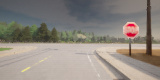
\includegraphics[width=\textwidth]{img/masking/object_detection/original.png}
    \caption{Original Image}
    \label{fig:orig}
\end{subfigure}
\hfill
\begin{subfigure}[b]{0.24\textwidth}
    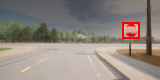
\includegraphics[width=\textwidth]{img/masking/object_detection/with_bbox.png}
    \caption{Object detected}
    \label{fig:orig_bbox}
\end{subfigure}
\hfill
\begin{subfigure}[b]{0.24\textwidth}
    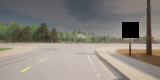
\includegraphics[width=\textwidth]{img/masking/object_detection/masked.png}
    \caption{Masked Image}
    \label{fig:masked}
\end{subfigure}
\hfill
\begin{subfigure}[b]{0.24\textwidth}
    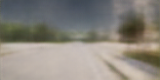
\includegraphics[width=\textwidth]{img/masking/object_detection/CE.png}
    \caption{Reconstructed Image}
    \label{fig:reconstructed}
\end{subfigure}
\caption{
Counterfactual generation through object detection-based masking in a CARLA driving scene. (a) The original image as captured. (b) A STOP sign is detected and localized using YOLOv5. (c) The STOP sign is masked by zeroing out its bounding box. (d) The masked image is reconstructed using a Variational Autoencoder (VAE). The classifier changes its prediction from \texttt{STOP} to \texttt{GO}, indicating that the STOP sign was a causally decisive feature in the original decision.
}
\label{fig:object_detection_masking}
\end{figure}


Figure~\ref{fig:object_detection_masking} illustrates a concrete example of the object detection based masking process applied to a realistic driving scenario. The scene was rendered in the CARLA simulator and contains a STOP sign located on the right-hand side of the road.

The unaltered version of the image (Figure~\ref{fig:orig}) corresponds to the model's original input, for which the classifier predicts the label \texttt{STOP} with high confidence. The YOLOv5 object detector accurately identifies and localizes the STOP sign (Figure~\ref{fig:orig_bbox}), represented by a red bounding box. This is a safety-critical decision, expected in the presence of a regulatory traffic sign.

To probe the causal influence of the STOP sign, the region corresponding to the bounding box is zeroed out (Figure~\ref{fig:masked}). This masked image is then passed through a decoder which reconstructs the image in a smooth and naturalistic manner (Figure~\ref{fig:reconstructed}). The reconstruction effectively blurs or removes the masked STOP sign, preserving the surrounding context to remain within the data manifold.

Upon re-encoding and classifying the reconstructed image, the model changes its decision from \texttt{STOP} to \texttt{GO}. This prediction flip signifies a valid counterfactual explanation. The STOP sign was a critical feature in the model’s decision process. Its removal induced a behavioral shift, indicating a direct causal pathway between the visual presence of the STOP sign and the predicted driving action.

This example validates the semantic sensitivity of the proposed method. It reveals that object detection-based masking can expose model dependencies on interpretable, high-level visual cues, facilitating transparency in AI-driven navigation systems. The corresponding results on this method and comparing the effectiveness to other methods are detailed in \cref{Evaluation and Results}.





\subsection{LIME on Image-Based Masking}
\label{sec:lime_on_images}

Local Interpretable Model-Agnostic Explanations (LIME) is an explainability technique that identifies input regions most responsible for a model’s prediction by perturbing the input and observing the resulting changes in output probabilities~\cite{Ribeiro2018}. For image data, LIME segments the input into superpixels and perturbs the image by masking these regions, then learns a local surrogate model to approximate the classifier’s decision boundary.

In our method, LIME is integrated into the counterfactual generation pipeline to evaluate whether removing highly influential visual regions can lead to a prediction flip. If the classifier changes its decision after masking the top-$k$ most important superpixels, the explanation is considered a valid counterfactual explanation (CE), indicating that the masked regions had a causal impact on the prediction.

We follow the unified masking pipeline described in Section~\ref{sec:feature_masking_pipeline}. First, the input image is passed through a Variational Autoencoder (VAE) to obtain a latent representation, which is then classified using a downstream classifier. LIME is applied to the \emph{raw input image} to compute a saliency mask highlighting the top-$k$ positively contributing superpixels (we use $k=5$), representing the most influential visual regions for the predicted class.

\begin{figure}[ht]
    \centering
    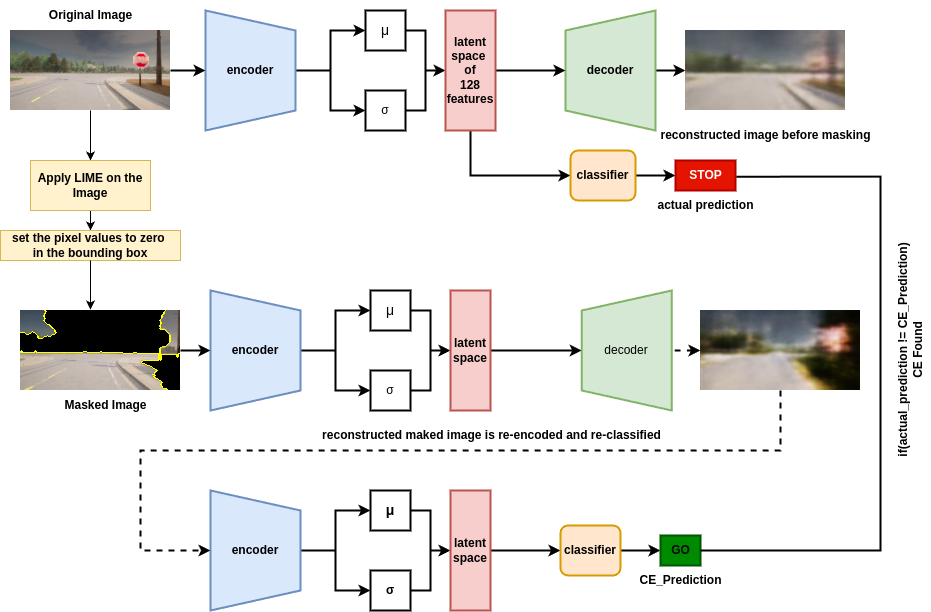
\includegraphics[width=0.95\textwidth]{img/masking/lime_on_images/lime_on_images_based_masking_flow.drawio.png}
    \caption{
    Workflow of the LIME-based counterfactual explanation pipeline. The input image is encoded using a VAE and classified to determine the original label (e.g., \texttt{STOP}). LIME is applied to the input image to identify the most influential superpixels. These regions are then hard-masked (blacked out), and the resulting image is passed through the encoder-decoder pipeline. The reconstructed image is re-encoded and re-classified. If the predicted class changes (e.g., from \texttt{STOP} to \texttt{GO}), a counterfactual explanation is found.
    }
    \label{fig:lime_image_workflow}
\end{figure}

To mask these regions, we adopt a hard masking strategy where the selected superpixels are replaced with a solid black color (i.e., pixel intensities set to zero). This masking approach is consistent with the strategies used in grid-based and object detection-based masking, promoting interpretability and ensuring uniformity across different masking techniques. The LIME-based masking operation can be formally expressed as:

\[
I_{\text{masked}} = I \odot (1 - M),
\]

where \( I \) is the original image, \( M \) is the binary LIME mask corresponding to the top-$k$ superpixels, and the masked image \( I_{\text{masked}} \) is generated by blacking out these regions.

Next, the masked image is passed through the VAE encoder to obtain a new latent representation, which is then decoded to reconstruct an image. This reconstructed image is re-encoded and classified again. If the predicted label changes at this stage, the masking is considered to have revealed a counterfactual explanation, indicating the causal importance of the masked regions.

Although LIME operates in the image space, the explanation it provides is ultimately linked to the classifier trained on the VAE’s latent representation. The prediction function passed to LIME includes two components: (i) encoding the perturbed image using the VAE encoder to obtain the latent vector, and (ii) passing this vector to the classifier to compute prediction probabilities. The decoder is only used after masking, to generate visually coherent reconstructions required for downstream evaluation. This end-to-end workflow is visually illustrated in Figure~\ref{fig:lime_image_workflow}, and the entire algorithmic process is outlined in Algorithm~\ref{alg:lime_on_images}.



\begin{algorithm}[ht]
\caption{LIME on Images for Counterfactual Generation (Hard Masking)}
\label{alg:lime_on_images}
\begin{algorithmic}[1]
\REQUIRE Image $I$, encoder $E$, decoder $D$, classifier $C$, LIME explainer $L$
\ENSURE Whether a counterfactual explanation is found

\STATE Encode image: $z \leftarrow E(I)$
\STATE Predict original label: $y_{\text{orig}} \leftarrow \arg\max C(z)$

\STATE Generate LIME explanation: $M \leftarrow L(I, C)$
\STATE Select top-$k$ regions: $R \leftarrow \text{Mask}(M, k=5)$
\STATE Apply hard masking: $I_{\text{masked}} \leftarrow I \odot (1 - R)$

\STATE Encode: $z_{\text{masked}} \leftarrow E(I_{\text{masked}})$
\STATE Decode: $I_{\text{recon}} \leftarrow D(z_{\text{masked}})$
\STATE Re-encode: $z_{\text{re}} \leftarrow E(I_{\text{recon}})$
\STATE Predict new label: $y_{\text{new}} \leftarrow \arg\max C(z_{\text{re}})$

\IF{$y_{\text{new}} \neq y_{\text{orig}}$}
    \RETURN Counterfactual explanation found
\ENDIF

\RETURN No counterfactual explanation found
\end{algorithmic}
\end{algorithm}

Compared to grid-based or object detection-based masking, LIME provides an \emph{adaptive and data-driven} approach to region selection. It focuses only on the most relevant image regions for a given prediction, enhancing interpretability and explanation quality. The corresponding results on this method and comparing the effectiveness to other methods are detailed in \cref{Evaluation and Results}.





\vspace{1em}
\subsection{LIME-Based Masking on Latent Features} \label{sec:lime_based_masking_on_latent_features}

\subsubsection*{Latent Feature Statistics Preprocessing}
\label{sec:latent_statistics_preprocessing}
Before applying LIME-based masking in the latent space, it is essential to establish dataset level statistical priors for each latent dimension. This ensures that when latent features are perturbed or replaced, the substituted values remain within a plausible range, preserving semantic consistency.

To compute these priors, all images from the training and test sets are encoded using the trained Variational Autoencoder (VAE) encoder, yielding a 128-dimensional latent vector for each image. The collection of these vectors across the dataset is used to compute per-dimension statistics, including the mean, median, minimum, maximum, and standard deviation.

These computed statistics are used during the masking phase to replace influential latent features. For instance, if LIME identifies a latent dimension as critical to the current classification, its value can be substituted with the median or mean value from the dataset to simulate a more neutral configuration. This strategy ensures that the modified latent vectors remain close to the data manifold, improving the realism of generated counterfactuals.

These statistics serve as the foundation for the LIME on Latent Features method and its Nearest Unchanged Neighbor (NUN) extension.


\subsection{LIME on Latent Features}
\label{sec:lime_on_latent}

This method applies the LIME (Local Interpretable Model-Agnostic Explanations) algorithm directly to the latent space of a trained Variational Autoencoder (VAE) to identify and mask the most influential latent dimensions contributing to the model's classification. Unlike image-space LIME, this approach operates on the compressed latent representation $z \in \mathbb{R}^{128}$, thereby enabling counterfactual reasoning at a more abstract and semantically meaningful level.

Prior to this step, dataset-level statistics such as the median of each latent dimension are computed and stored, as described in Section~\ref{sec:latent_statistics_preprocessing}. These median values, denoted as $\bar{z} \in \mathbb{R}^{128}$, are used as neutral replacements for feature masking.

As shown in the workflow in Figure~\ref{fig:lime_latent_workflow}, the VAE encoder maps the input image $I$ into a latent representation $z = E(I)$. A downstream neural classifier $C$ then provides the prediction $\hat{y}_{\text{orig}} = \arg\max C(z)$. LIME is applied on this latent vector to compute a local linear approximation of the classifier’s decision boundary and returns a list of tuples $\{(w_i, i)\}$, where $w_i$ is the importance weight of the $i$-th latent feature.

\begin{figure}[htbp]
\centering
    \begin{subfigure}{0.24\textwidth}
        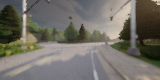
\includegraphics[width=\linewidth]{img/masking/lime_on_latent/original.png}
        \caption*{(a) Original image}
        \end{subfigure}
    \hfill
    \begin{subfigure}{0.72\textwidth}
        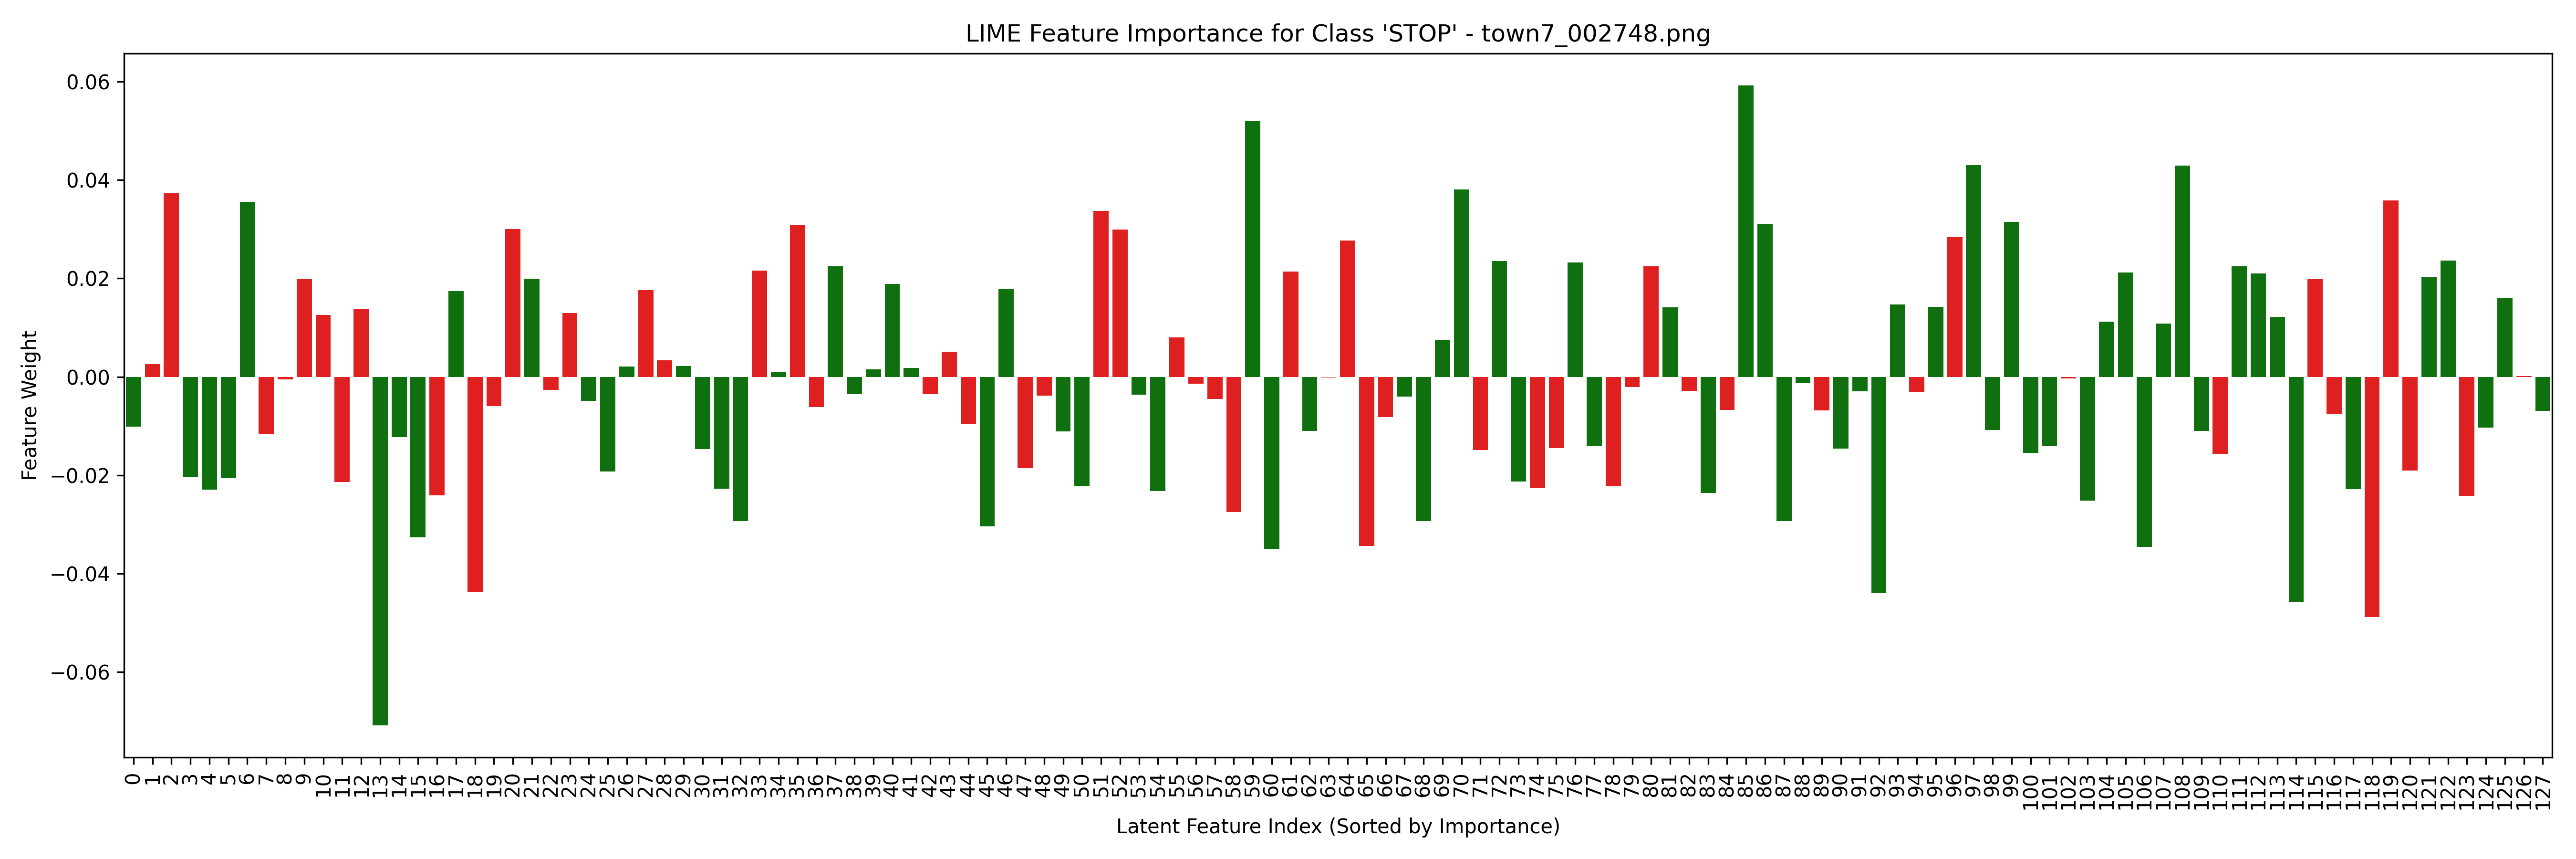
\includegraphics[width=\linewidth]{img/masking/lime_on_latent/town7_002748.png_lime_feature_importance_class_STOP_sorted.png}
        \caption*{(b) LIME importance plot for class \texttt{STOP}, with both weight}
    \end{subfigure}
    \vspace{0.5em}
    \begin{subfigure}{0.72\textwidth}
        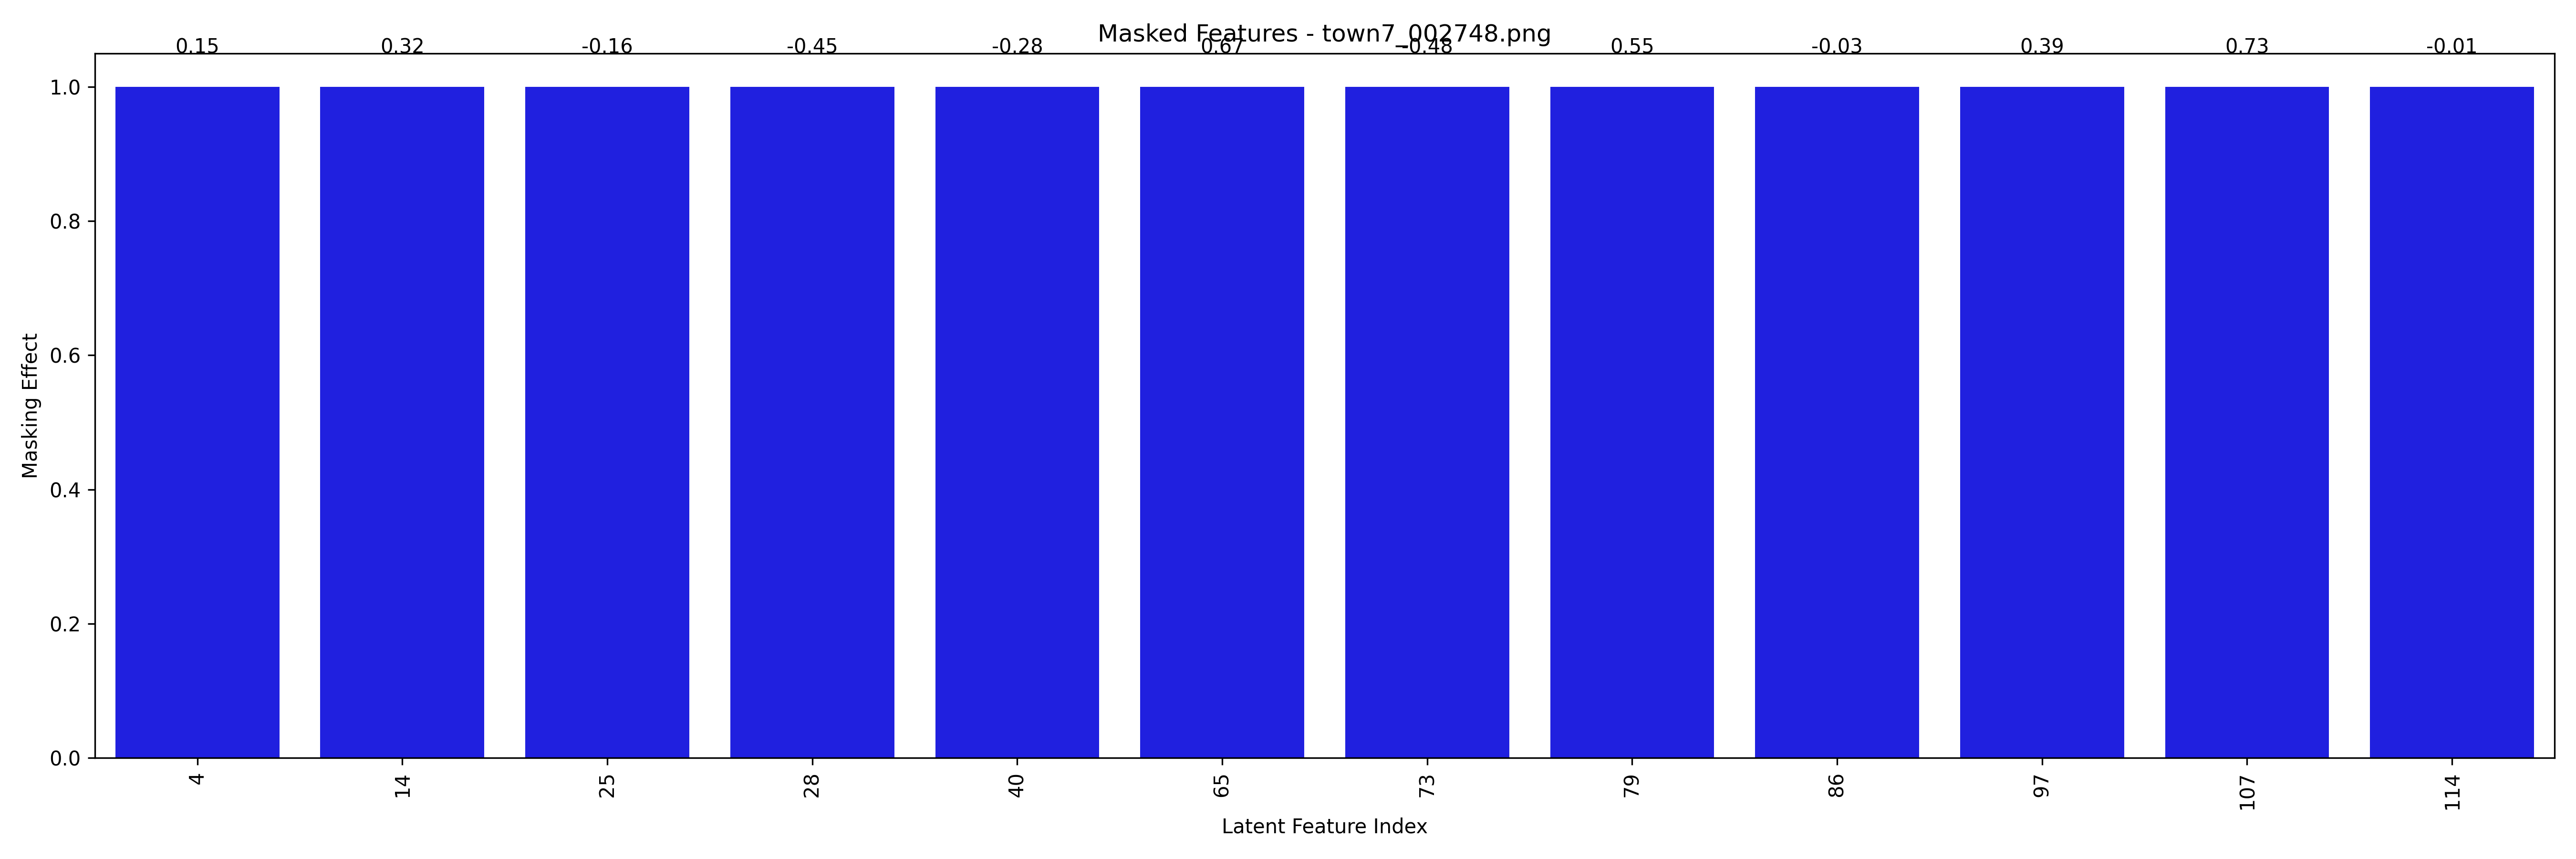
\includegraphics[width=\linewidth]{img/masking/lime_on_latent/town7_002748.png_masked_features.png}
        \caption*{(c) Features masked using median values and their LIME weights}
    \end{subfigure}
    \hfill
    \begin{subfigure}{0.24\textwidth}
        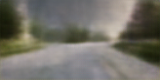
\includegraphics[width=\linewidth]{img/masking/lime_on_latent/reconstructed_lime_on_features.png}
        \caption*{(d) Reconstructed image after LIME-based masking}
    \end{subfigure}

    \caption{LIME on Latent Space Masking: The original image was classified as STOP (confidence: 52.5\%). LIME identified positively contributing latent features, which were progressively replaced by their corresponding dataset-level median values. The prediction flipped to RIGHT (confidence: 48.3\%) after masking 12 features, as seen in the reconstructed image. In the LIME plot, red bars indicate features positively influencing the original prediction, while green bars indicate negative influence. The removed features likely correspond to visual elements such as traffic signals, making the reconstructed image appear navigable toward the right. A detailed analysis is provided in \cref{Evaluation and Results}}.


\end{figure}

Only the positively influential features (i.e., $w_i > 0$) are considered for masking, as shown in the sorted LIME importance plot (Figure~\ref{fig:lime_latent_example}b). This choice ensures that we are suppressing features that actively contribute toward the current classification. Replacing negatively influential features (those working against the current class) would potentially reinforce the current decision and thus contradict the goal of counterfactual generation.

The positively weighted features are sorted in descending order of importance, i.e., from the most impactful dimension to the least (Figure~\ref{fig:lime_latent_example}b). Let $\mathcal{F} = \{i_1, i_2, \dots, i_k\}$ denote the ordered set of positively contributing latent feature indices. For each $i \in \mathcal{F}$, the feature $z_i$ is replaced by the corresponding dataset-level median $\bar{z}_i$:


\[
z_i^{\text{masked}} = 
\begin{cases}
\bar{z}_i & \text{if } i \in \mathcal{F}_{\text{used}} \\
z_i & \text{otherwise}
\end{cases}
\]

The modified latent vector is then passed through the decoder to reconstruct an image $I_{\text{recon}} = D(z^{\text{masked}})$ (Figure~\ref{fig:lime_latent_example}c). This image is re-encoded and classified again to obtain a new prediction $\hat{y}_{\text{new}} = \arg\max C(E(I_{\text{recon}}))$. If $\hat{y}_{\text{new}} \ne \hat{y}_{\text{orig}}$, the explanation is accepted as a valid counterfactual explanation. The corresponding LIME weights and masked features are visualized in Figure~\ref{fig:lime_latent_example}(d).



\begin{figure}[h]
    \centering
    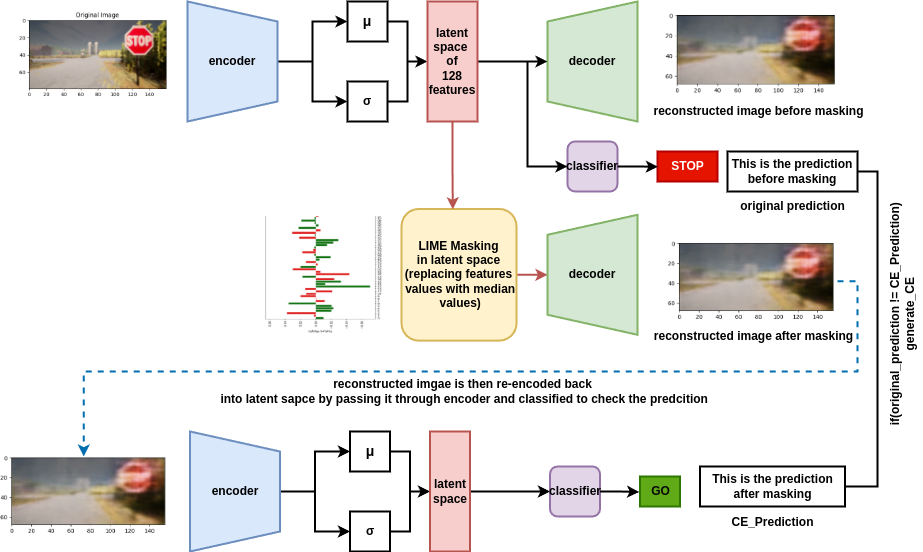
\includegraphics[width=0.95\linewidth]{img//masking/lime_on_latent/LIME_on_latent_space_masking.png}
    \caption{Workflow of the LIME-based masking method applied in the latent space of a Variational Autoencoder (VAE). 
    The input image is first encoded to a 128-dimensional latent vector. A classifier trained on the latent space predicts the original label (e.g., \texttt{STOP}). 
    LIME is used to determine the top contributing latent features towards this prediction. These features are replaced one by one with their corresponding dataset-level median values (precomputed and stored). 
    Each masked latent vector is decoded to reconstruct a perturbed image, which is then re-encoded and re-classified. 
    If the classifier prediction changes (e.g., to \texttt{GO}), a counterfactual explanation is recorded. 
    The process leverages statistical feature replacement to ensure semantic plausibility, and early stopping is used to identify the minimal set of influential latent dimensions required to flip the decision.
    }
    \label{fig:lime_latent_workflow}
\end{figure}

The full procedure is detailed in Algorithm~\ref{alg:lime_on_latent}, and the complete masking pipeline is illustrated in Figure~\ref{fig:lime_latent_workflow}. This approach ensures semantic plausibility by leveraging dataset-informed statistics and offers a high-level explanation by manipulating deep features learned through the VAE.


\vspace{1em}
\begin{algorithm}[H]
\caption{LIME-Based Masking on Latent Features}
\label{alg:lime_on_latent}
\begin{algorithmic}[1]
\REQUIRE Image $I$, encoder $E$, decoder $D$, classifier $C$, median latent vector $\bar{z}$
\ENSURE Whether a counterfactual explanation is found

\STATE $z \leftarrow E(I)$ \hfill // Encode image to latent vector
\STATE $y_{\text{orig}} \leftarrow \arg\max C(z)$ \hfill // Original prediction

\STATE Use LIME to compute feature importance scores on $z$
\STATE Select positively influential features $\mathcal{F}$, sorted by importance
\FOR{feature index $i$ in $\mathcal{F}$}
    \STATE $z_{\text{masked}} \leftarrow z$ with $z_i \leftarrow \bar{z}_i$
    \STATE $I_{\text{recon}} \leftarrow D(z_{\text{masked}})$
    \STATE $z_{\text{re}} \leftarrow E(I_{\text{recon}})$
    \STATE $y_{\text{new}} \leftarrow \arg\max C(z_{\text{re}})$
    \IF{$y_{\text{new}} \neq y_{\text{orig}}$}
        \RETURN Counterfactual explanation found
    \ENDIF
\ENDFOR

\RETURN No counterfactual explanation found
\end{algorithmic}
\end{algorithm}
\vspace{1em}

This method provides a more abstract yet powerful mechanism for generating counterfactuals, as it operates on high-level learned features. The use of dataset-informed median values ensures semantic consistency, while early stopping improves efficiency. Interpretability is further enhanced by generating visualizations such as LIME importance bar plots and masked feature maps, and effectiveness and performance comparasion with other masking methods are discussed in the \cref{sec:masking_eval}.





\subsection{LIME-Guided Latent Feature Masking using NUN} \label{lime_with_NUN}

In this work, we extend the counterfactual explanation strategy introduced by Wijekoon et al.~\cite{WijekoonWNMPC21} to the domain of deep generative models. While originally applied to tabular data, we adapt their approach to the latent space of image representations learned by a Variational Autoencoder (VAE) which is again a tabular data. Specifically, we implement Method 2, in which LIME a post-hoc method is applied to the latent vector of a \textit{Nearest Unlike Neighbor} (NUN) to guide feature replacement in the query representation until a class change is achieved.

Given an input image \( x \), we encode it into a latent vector \( z \) using a pretrained VAE encoder \( E \), and obtain its predicted class \( y = \arg\max C(z) \) from a trained classifier \( C \). We then identify the Nearest Unlike Neighbor \( \hat{z} \), which belongs to a different predicted class \( \hat{y} \ne y \), by computing the Euclidean distance in the latent space:

\[
\hat{z} = \arg\min_{z_j \in \mathcal{D}_{\text{test}}} \left\{ \| z - z_j \|_2 \; \middle| \; C(z_j) \ne y \right\}
\]

This NUN latent vector represents a semantically similar example that yields a different classification, and thus serves as a candidate for counterfactual explanation generation.

To prioritize the most relevant feature changes, we apply the \textit{LIME Tabular Explainer}~\cite{Ribeiro2018} to the NUN vector \( \hat{z} \). LIME generates a local surrogate model that assigns importance weights to each latent feature, resulting in an ordered list:

\[
\text{AFOrderLIME}(\hat{z}) = \{ i_1, i_2, \dots, i_m \}, \quad \text{where } |w_{i_1}| > |w_{i_2}| > \dots > |w_{i_m}|
\]

These weights reflect how much each latent feature contributes to the predicted class of the NUN. We use this ranking to iteratively transfer features from \( \hat{z} \) to the query vector that is input image vector\( z \).

Following the LIME importance order, each dimension is replaced via \( z[i_k] \leftarrow \hat{z}[i_k] \), and the modified latent vector \( z' \) is reconstructed into an image \( x' = D(z') \). The reconstructed image is re-encoded and re-classified to determine whether a class change has occurred. This process continues until the prediction flips, identifying a minimal set of latent features required to finding a counterfactual explanation. The complete procedure is summarized in Algorithm~\ref{alg:nun_lime} and the workflow is is shown in Figure~\ref{fig:nun_lime}

\begin{figure}[htbp]
    \centering
    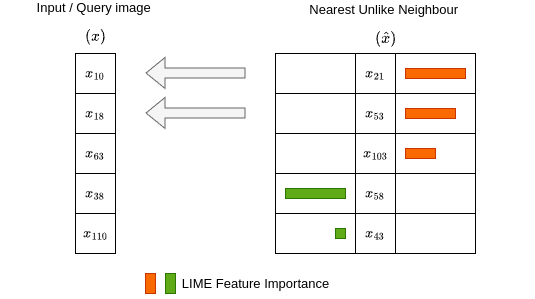
\includegraphics[width=0.55\textwidth]{img/masking/lime_on_latent_nun/NUN_method.drawio.png}
    \caption{Illustration of the proposed method. Important latent features (as determined by LIME) are transferred from the NUN to the input in order of decreasing importance until the classifier's prediction changes.}
    \label{fig:nun_lime}
\end{figure}


\begin{figure}[htbp]
    \centering
    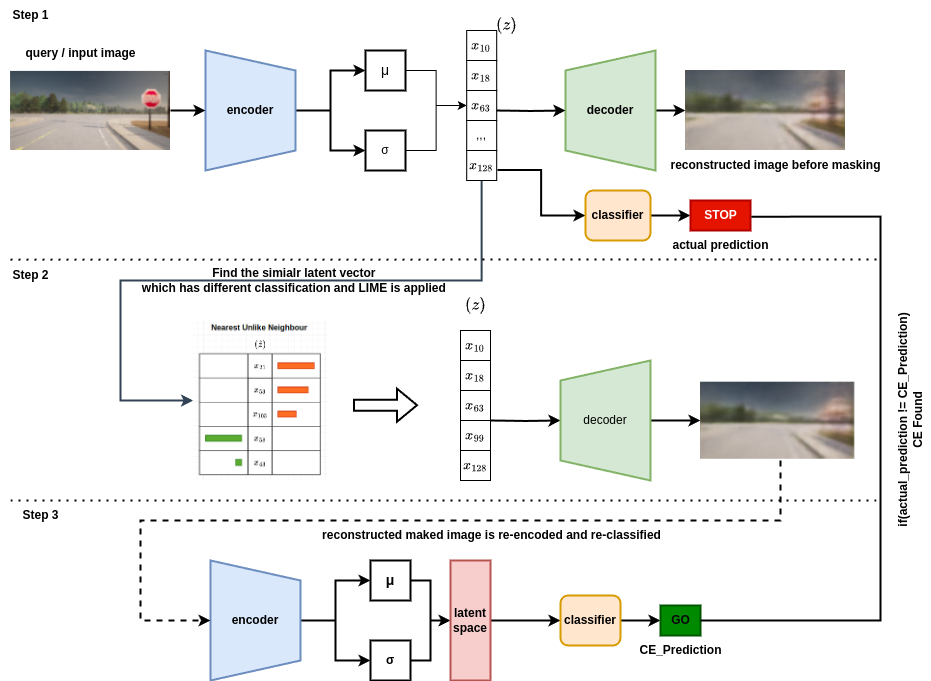
\includegraphics[width=0.95\textwidth]{img/masking/lime_on_latent_nun/lime_on_latent_featuring_using_NUN.png}
    \caption{
    Workflow of the LIME-Guided Latent Feature Masking using Nearest Unlike Neighbor (NUN). 
    Step 1: The query image is encoded into a 128-dimensional latent vector using the VAE encoder and classified to obtain the original prediction (\texttt{STOP}).  
    Step 2: A latent vector from the test set with a different class prediction (NUN) is selected based on Euclidean proximity. LIME is applied to the NUN to rank the most influential latent features contributing to its class. These top-k features are iteratively transferred from the NUN to the query latent vector.  
    Step 3: After each replacement, the latent vector is decoded to an image, re-encoded, and re-classified. If the prediction changes (e.g., to \texttt{GO}), the replaced features are considered causally decisive, and the outcome is recorded as a counterfactual explanation.
    }
    \label{fig:nun_lime}
\end{figure}


An illustration of this feature transfer mechanism is shown in Figure~\ref{fig:nun_lime}. The left column depicts the latent features of the input image, while the right column represents the features of its NUN. LIME-assigned importance is indicated through color-coded bars. Features with higher importance are prioritized during transfer from the NUN to the query. Arrows between the two vectors highlight the flow of values during the masking process.


\begin{figure}
    \centering
    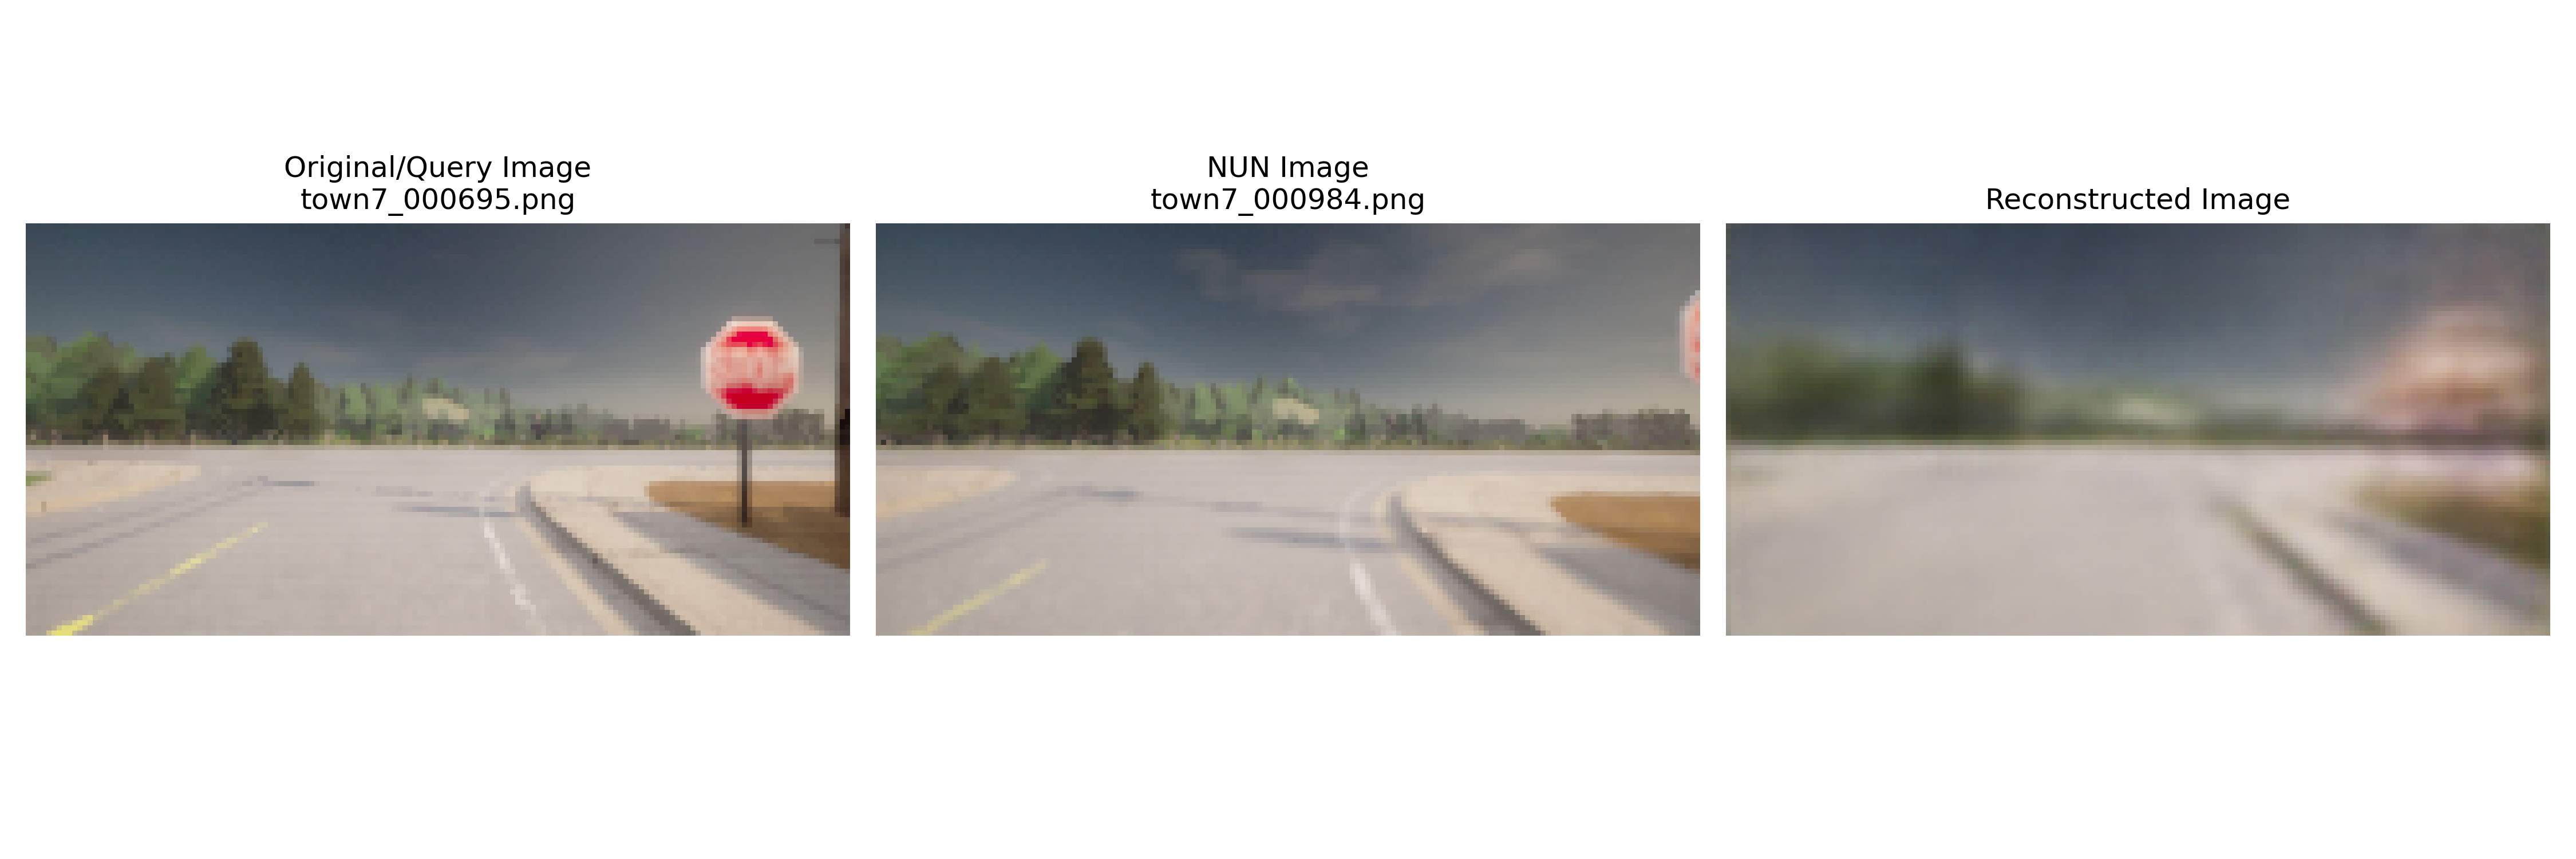
\includegraphics[width=1\linewidth]{img//masking//lime_on_latent_nun/town7_000695.png_side_by_side.png}
    \caption{
    This is Visual Comparison of LIME guided Latent feature masking using Nearest Unlike Neighbor(NUN) with respect to input image of my dataset. LEFT: Example of the query image which is first classified as STOP. NUN is derived from a semantically similar image (middle), but classified as GO. Right: The reconstructed image where counterfactual explanation is found.
    }
    \label{fig:nun_cf_side_by_side}
\end{figure}


\begin{algorithm}[htbp]
\caption{LIME-Based Masking on Latent Features using NUN}
\label{alg:nun_lime}
\begin{algorithmic}[1]
\REQUIRE Encoder $E$, Decoder $D$, Classifier $C$, Query image $I$, Test dataset $\mathcal{D}_{\text{test}}$, Label mapping $\mathcal{L}$
\ENSURE Counterfactual image $x_{\text{cf}}$, Number of features replaced $k$, Evaluation metrics

\STATE $z \leftarrow E(I)$ \hfill \textit{// Encode query to latent space}
\STATE $y \leftarrow \arg\max C(z)$ \hfill \textit{// Get predicted label}
\STATE $z_{\text{NUN}} \leftarrow \text{None}$, $d_{\min} \leftarrow \infty$

\FORALL{$J \in \mathcal{D}_{\text{test}}$}
    \STATE $z_j \leftarrow E(J)$
    \STATE $y_j \leftarrow \arg\max C(z_j)$
    \IF{$y_j \ne y$}
        \STATE $d \leftarrow \|z - z_j\|_2$
        \IF{$d < d_{\min}$}
            \STATE $z_{\text{NUN}} \leftarrow z_j$
            \STATE $d_{\min} \leftarrow d$
        \ENDIF
    \ENDIF
\ENDFOR

\STATE $\text{importance} \leftarrow \text{LIME}(z_{\text{NUN}}, C)$
\STATE $\mathcal{F} \leftarrow \text{SortDescendingByImportance}(\text{importance})$
\STATE $z_{\text{mod}} \leftarrow z$, $k \leftarrow 0$

\FORALL{$i \in \mathcal{F}$}
    \STATE $z_{\text{mod}}[i] \leftarrow z_{\text{NUN}}[i]$
    \STATE $x_{\text{recon}} \leftarrow D(z_{\text{mod}})$
    \STATE $z_{\text{reenc}} \leftarrow E(x_{\text{recon}})$
    \STATE $y_{\text{new}} \leftarrow \arg\max C(z_{\text{reenc}})$
    \STATE $k \leftarrow k + 1$
    \IF{$y_{\text{new}} \ne y$}
        \STATE \textbf{break}
    \ENDIF
\ENDFOR

\STATE $\text{metrics} \leftarrow \text{Evaluate}(I, x_{\text{recon}})$
\RETURN $x_{\text{recon}}, k, \text{metrics}$
\end{algorithmic}
\end{algorithm}


This approach leverages LIME’s interpretability and the semantic richness of the latent space to generate actionable counterfactuals. It ensures minimal intervention while maintaining high visual fidelity, and directly aligns with the counterfactual generation principles outlined by Wijekoon et al.~\cite{WijekoonWNMPC21}. The corresponding results on this method and comparing the effectiveness to other methods are detailed in \cref{sec:masking_eval}.









\chapter{Evaluation and Results} \label{Evaluation and Results}
repeate th RQs


\subsection{Evaluation of Variational Autoencoder (VAE)} \label{subsec:vae_evaluation}
To assess the effectiveness of the trained Variational Autoencoder (VAE) in learning meaningful latent representations and high-quality image reconstructions, a combination of quantitative and qualitative evaluations was performed. Two reconstruction losses Mean Squared Error (MSE) and Log-Cosh were compared to determine their impact on training dynamics and final reconstruction quality. The evaluation spans across total loss, reconstruction fidelity, KL divergence behavior, perceptual quality (PSNR), pixel-level accuracy, and visual inspection of reconstructed samples.

\subsubsection{Quantitative Evaluation}
To assess the performance of the Variational Autoencoder (VAE), both the Log-Cosh and Mean Squared Error (MSE) loss functions were evaluated across several metrics, namely Total Loss, Reconstruction Loss, KL Divergence, Validation Pixel Accuracy, Peak Signal-to-Noise Ratio (PSNR). 

The following table summarizes the average values over the final 5 epochs for both models:

\begin{table}[h]
    \centering
    \begin{tabular}{lcc}
        \toprule
        \textbf{Metric} & \textbf{Log-Cosh (Final Avg)} & \textbf{MSE (Final Avg)} \\
        \midrule
        Validation Total Loss & 21.82 & 42.35 \\
        Validation Recon Loss & 16.49 & 35.84 \\
        Validation KL Divergence & 268.72 & 327.90 \\
        Validation Pixel Accuracy & 0.971 & 0.969 \\
        Validation PSNR (dB) & 31.39 & 30.99 \\
        \bottomrule
    \end{tabular}
    \caption{Average values over the final 5 epochs for Log-Cosh and MSE loss functions.}
    \label{tab:vae_evaluation}
\end{table}

From these results:

\begin{itemize}
    \item The Log-Cosh loss achieves significantly lower total and reconstruction loss.
    \item It also yields a higher PSNR, indicating better perceptual quality.
    \item Pixel accuracy is slightly better with Log-Cosh as well.
    \item Interestingly, the KL divergence is higher for MSE, indicating possible over-regularization.
\end{itemize}






\subsection{Neural Classifier on Latent Features (4-Class)}

To evaluate the performance of the neural network classifier trained on VAE-extracted latent features, both quantitative metrics and qualitative visualizations were analyzed.

The model was trained for 20 epochs in the 4-class dataset (\texttt{STOP}, \texttt{GO}, \texttt{RIGHT}, \texttt{LEFT}) using the training set of 13,308 samples and evaluated on a held-out test set of 3,284 samples. The training progression is shown in Figure~\ref{fig:loss_accuracy_plot}.

\begin{figure}[h]
    \centering
    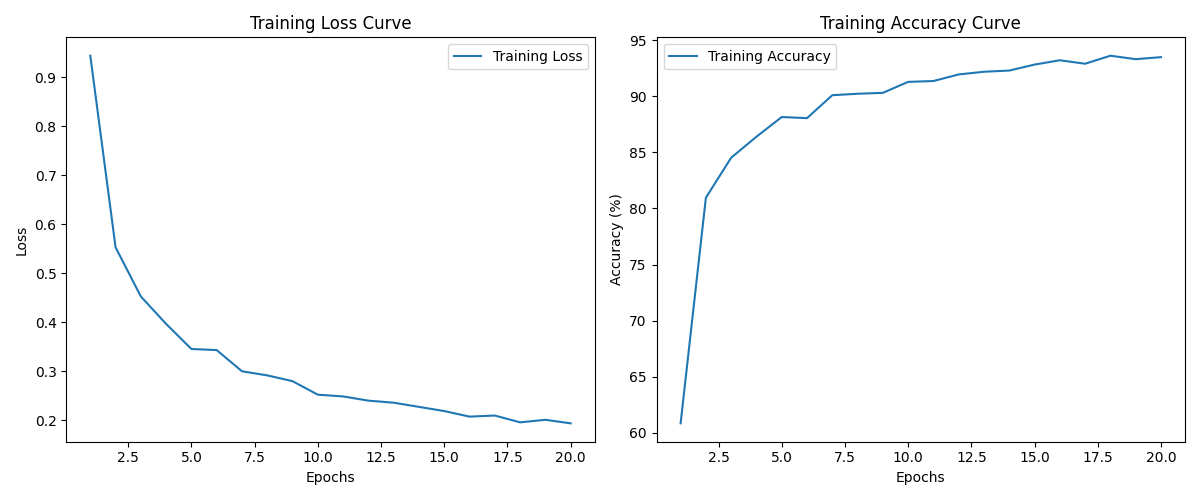
\includegraphics[width=\textwidth]{img/classifier/training_loss_accuracy_4_classes.png}
    \caption{Training loss and accuracy curves for the neural classifier.}
    \label{fig:loss_accuracy_plot}
\end{figure}

The training curves indicate a steady decrease in loss and improvement in accuracy, reaching a final training accuracy of approximately 89.4\%. This suggests the model learned meaningful patterns from the latent features without overfitting.

\subsubsection*{Classification Report}

Table~\ref{tab:classification_report} summarizes the classifier's performance on each class using precision, recall, and F1-score:

\begin{table}[h]
\centering
\begin{tabular}{lcccc}
\toprule
\textbf{Class} & \textbf{Precision} & \textbf{Recall} & \textbf{F1-score} & \textbf{Support} \\
\midrule
STOP  & 0.91 & 0.99 & 0.95 & 821 \\
GO    & 0.81 & 0.84 & 0.83 & 821 \\
RIGHT & 0.93 & 0.86 & 0.89 & 821 \\
LEFT  & 0.93 & 0.89 & 0.91 & 821 \\
\midrule
\textbf{Accuracy} & \multicolumn{4}{c}{0.89 (3284 samples)} \\
\textbf{Macro avg} & 0.90 & 0.89 & 0.89 & -- \\
\textbf{Weighted avg} & 0.90 & 0.89 & 0.89 & -- \\
\bottomrule
\end{tabular}
\caption{Classification report for the neural classifier (4-class).}
\label{tab:classification_report}
\end{table}

\subsubsection*{Confusion Matrix}

The confusion matrix in Figure~\ref{fig:conf_matrix} provides further insight into class-wise misclassifications:

\begin{figure}[h]
    \centering
    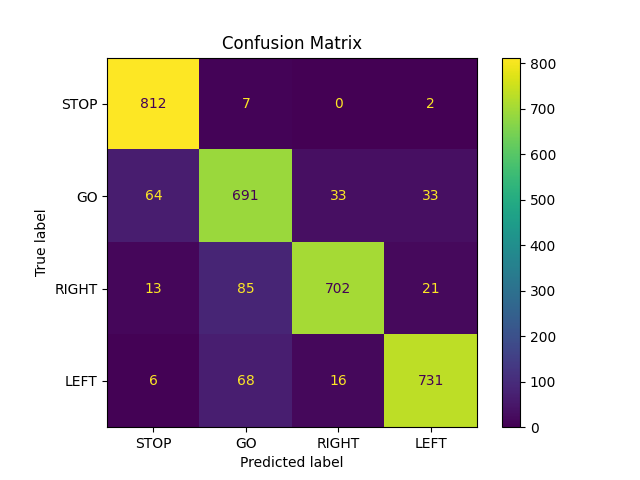
\includegraphics[width=0.6\textwidth]{img/classifier/confusion_matrix_4_classes.png}
    \caption{Confusion matrix for the neural classifier on the 4-class test set.}
    \label{fig:conf_matrix}
\end{figure}

\textbf{Observations:}
\begin{itemize}
    \item \textbf{STOP:} Most accurately classified class with a recall of 0.99.
    \item \textbf{GO:} Relatively weaker precision and recall; misclassified as \texttt{RIGHT} or \texttt{LEFT} in 8\% of cases.
    \item \textbf{RIGHT:} High precision, but some overlap with \texttt{GO} (85 misclassifications).
    \item \textbf{LEFT:} Very strong performance overall, with some confusion with \texttt{GO}.
\end{itemize}

These results confirm that the classifier is highly capable of distinguishing most driving actions using VAE latent features, though the \texttt{GO} class remains the most ambiguous.




\subsection{Comparison with Traditional Classifiers}

To contextualize the performance of the neural network classifier, a suite of traditional machine learning models were trained and evaluated on the same latent feature representations extracted from the VAE. These models include Logistic Regression, K-Nearest Neighbors (KNN), Support Vector Machine (SVM), and Random Forest. Each model was trained on the 128-dimensional latent vectors and tested on the same 4-class dataset.

Table~\ref{tab:classifier_comparison} presents a side-by-side comparison of accuracy and F1-scores across all classifiers:

\begin{table}[h]
\centering
\small 
\begin{tabular}{p{2.5cm}ccp{3.5cm}}
\toprule
\textbf{Classifier} & \textbf{Accuracy} & \textbf{Macro F1} & \textbf{Notes} \\
\midrule
Logistic Regression & 80\% & 0.80 & Baseline linear classifier; struggled with \texttt{GO} \\[2pt]
KNN & 88\% & 0.88 & High recall for \texttt{STOP}, sensitive to latent proximity \\[2pt]
SVM & 89\% & 0.89 & Excellent class separability; especially for \texttt{LEFT} and \texttt{STOP} \\[2pt]
Random Forest & 88\% & 0.88 & Robust performance; most errors in \texttt{GO} class \\[2pt]
Neural Network & \textbf{89\%} & \textbf{0.89} & Best overall F1 balance; handles non-linear separations \\
\bottomrule
\end{tabular}
\caption{Performance comparison of classifiers trained on VAE latent features (4-class).}
\label{tab:classifier_comparison}
\end{table}

\textbf{Key Observations:}
\begin{itemize}
    \item The neural classifier and SVM achieved the highest overall accuracy and macro F1-score (both 0.89), indicating strong class separation in the latent space.
    \item Logistic Regression performed the weakest, highlighting the limitation of linear decision boundaries in this latent representation.
    \item KNN and Random Forest both achieved strong results, particularly for the \texttt{STOP} class, but showed more confusion on the \texttt{GO} class.
    \item Across all models, the \texttt{GO} class consistently had the lowest precision and recall, suggesting overlapping representations in the latent space that merit further exploration.
\end{itemize}

These results confirm the value of the VAE latent space as a compact and expressive representation, allowing both deep and traditional classifiers to achieve competitive performance on complex multi-class driving data.



\section{Evaluation of Masking Methods} \label{sec:evaluation}
To address \textbf{RQ3} (see Section~\ref{sec:research_question}), we performed a comprehensive evaluation of all implemented masking techniques across multiple dimensions: counterfactual coverage, computational efficiency, method overlap, and robustness. A custom Python script was developed to automate the analysis by aggregating and comparing the results from each method's output CSV files.

The script computes the total number of counterfactual explanations (CEs) found per method, their distribution across class labels, and the overall time taken. It also generates:

\begin{itemize}
    \item \textbf{Venn diagrams} illustrating overlaps in images where different methods found CEs,
    \item \textbf{Bar charts} summarizing the count of successful explanations,
    \item \textbf{Comparison tables} detailing which images were explained by which method,
    \item \textbf{Overlap summaries} categorizing all images based on individual or shared method success,
    \item \textbf{Sanity checks} verifying consistency and correctness in prediction changes,
    \item \textbf{Validity checks} ensuring the reconstructed images are plausible (via SSIM, PSNR, etc.).
\end{itemize}

These results are saved as CSV and high-resolution plots and are discussed in detail in Section~\ref{sec:results_and_discussion}.




\section{Overview of the Evaluation Strategy}
Counterfactuals were evaluated using both AI-based metrics and human evaluation.

\section{AI-Based Quantitative Evaluation}

\subsection{Evaluating the VAE Reconstruction Performance}
traditional loss like MSE loss vs logcosh loss comparison.
The SSIM and PSNR scores were computed to measure the quality of image reconstructions.
A visualization of reconstructed vs. original images was analyzed.

To evaluate the quality of the counterfactual explanations generated by our three methods: 
\textbf{Grid-Based Masking, LIME on Images, LIME on Latent Features}, we collected user ratings based on three criteria: 
\textbf{Interpretability, Plausibility, Visual Coherence}. Users rated each counterfactual on a scale of 1 (poor) to 5 (excellent). 
The collected data were stored in a CSV file, and we computed the mean ratings for each method and criterion.


\subsection{Counterfactual Success Rate (CSR) Across Different Masking Methods}
CSR measures how often a counterfactual successfully flips the classifier’s decision.
Comparison of CSR across different masking methods:
LIME on Latent Features: X%
Grid-Based Masking: Y%
Object Detection-Based Masking: Z%
LIME on Images: W%


\subsection{Structural and Visual Quality of Counterfactuals}
SSIM and PSNR were computed for counterfactual images to assess realism.






\section{Human Evaluation of Counterfactual Explanations} \label{section:Human Evaluation of Counterfactual Explanations}

\subsection{Study Setup and Procedure}
Participants were presented with counterfactual images generated by different masking techniques.
They were asked to select the most preferred counterfactual explanation based on:
Interpretability
Plausibility
Visual Coherence

\subsection{User Preferences for Different Masking Methods}
Percentage of participants preferring each method was analyzed.


\subsection{Correlation Between Human Preferences and AI-Based Metrics}
The relationship between human-selected best counterfactuals and AI-based evaluation scores (CSR, SSIM, PSNR) was analyzed.




\subsection{Quantitative Analysis}
\label{subsec:quantitative_analysis}

Our design aligns with insights from Delaney et al.~\cite{DELANEY2023103995}, who argue that evaluation of counterfactuals should reflect human explanation goals. They show that traditional metrics like L1/L2 distance are often misaligned with human expectations of plausibility. Accordingly, we incorporate both quantitative metrics validity and a human rating study focused on interpretability, Plausibility, and Visual Coherence and semantic consistency.

Figure~\ref{fig:barPlotAll} shows a combined bar chart comparing average ratings for Interpretability, Plausibility, and Visual Coherence 
across the three counterfactual methods. Meanwhile, Figure~\ref{fig:heatmap} provides a heatmap visualization for these metrics, 
making it easy to compare each method's performance at a glance.

\begin{figure}[htbp]
    \centering
    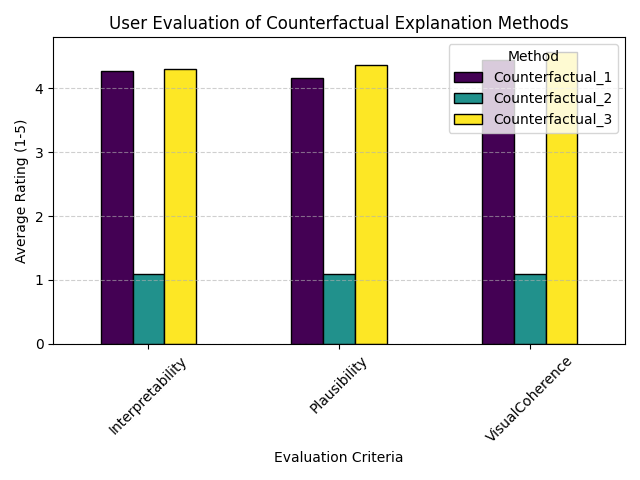
\includegraphics[width=0.7\textwidth]{img/results/bar_plot_user_evaluations.png}
    \caption{User Evaluation of Counterfactual Explanation Methods: Combined Bar Chart}
    \label{fig:barPlotAll}
\end{figure}

\begin{figure}[htbp]
    \centering
    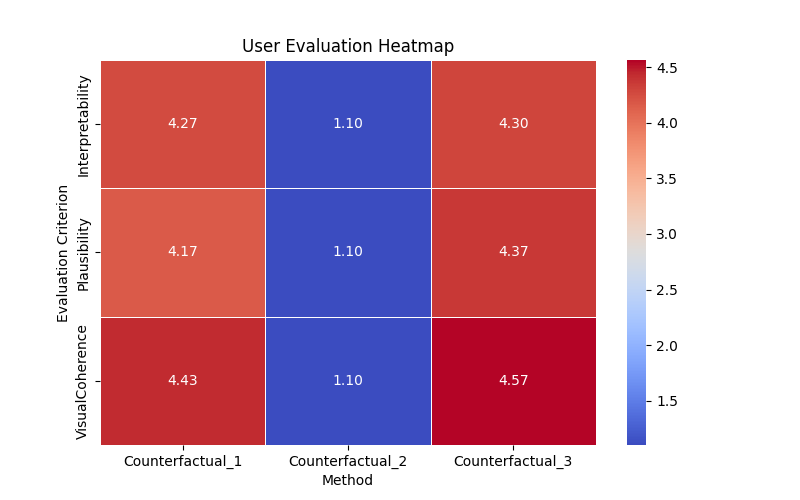
\includegraphics[width=0.7\textwidth]{img/results/heatmap_user_evaluations.png}
    \caption{User Evaluation Heatmap for Three Counterfactual Methods}
    \label{fig:heatmap}
\end{figure}

In addition to these combined views, we generated individual bar charts for each criterion (Figures~\ref{fig:interpretabilityBar}, 
\ref{fig:plausibilityBar}, and \ref{fig:visualCoherenceBar}). Each figure focuses on one metric and plots the average rating 
for each counterfactual method.

\begin{figure}[htbp]
    \centering
    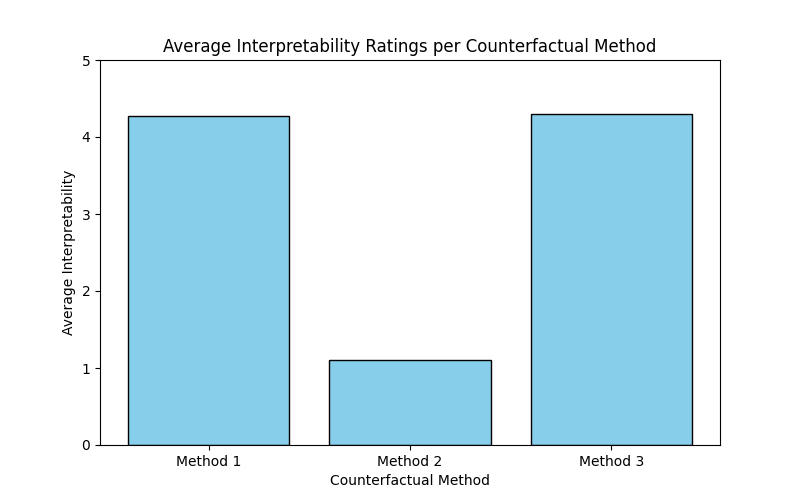
\includegraphics[width=0.55\textwidth]{img/results/Interpretability_ratings.png}
    \caption{Average Interpretability Ratings per Counterfactual Method}
    \label{fig:interpretabilityBar}
\end{figure}

\begin{figure}[htbp]
    \centering
    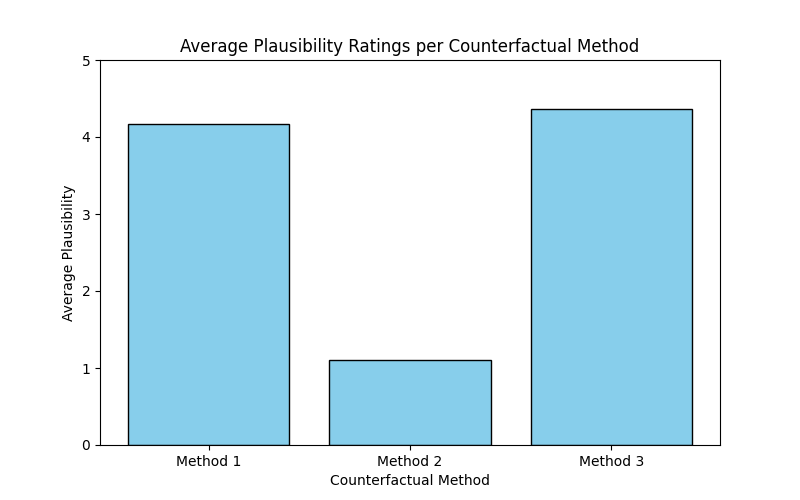
\includegraphics[width=0.55\textwidth]{img/results/Plausibility_ratings.png}
    \caption{Average Plausibility Ratings per Counterfactual Method}
    \label{fig:plausibilityBar}
\end{figure}

\begin{figure}[htbp]
    \centering
    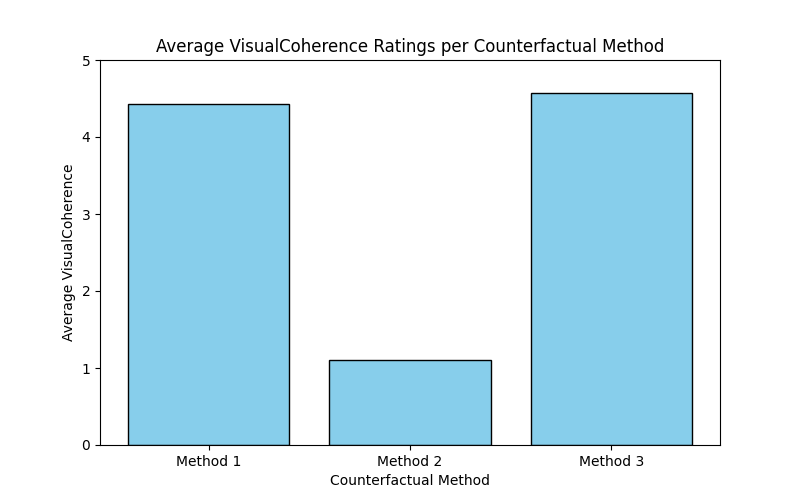
\includegraphics[width=0.55\textwidth]{img/results/VisualCoherence_ratings.png}
    \caption{Average Visual Coherence Ratings per Counterfactual Method}
    \label{fig:visualCoherenceBar}
\end{figure}

Overall, these visualizations indicate that \textbf{Method 3} achieves the highest scores across most metrics, particularly in 
\textit{Visual Coherence} and \textit{Interpretability}, while \textbf{Method 2} often lags behind in \textit{Plausibility} and 
\textit{Visual Coherence}. \textbf{Method 1} offers moderate-to-high performance in most categories but does not surpass Method 3.

\section{Validity}
\label{sec:validity}
Validity is a measure of how often the counterfactual explanation is successfully generated. 
The validity percentage is computed as
\[
\text{Validity (\%)} = \left( \frac{\text{Successful Counterfactuals}}{\text{Total Counterfactuals}} \right) \times 100.
\]

For our methods, a counterfactual is considered valid if it changes the model’s predic-
tion to the desired target class (e.g., from STOP to GO, or from RIGHT to LEFT). 

Table~\ref{tab:validity_results} summarizes the validity results obtained from four different methods:

\begin{table}[htbp]
    \centering
    \caption{Validity of Counterfactual Explanations}
    \label{tab:validity_results}
    \begin{tabular}{lcccc}
        \hline
        \textbf{Method} & \textbf{Total} & \textbf{Successful} & \textbf{Validity (\%)} \\
        & \textbf{Counterfactuals} & \textbf{Counterfactuals} & \\
        \hline
        Grid-Based Masking & 2326 & 2316 & 99.57 \\
        Object Detection & 2326 & 84 & 3.61 \\
        LIME on Images & 2326 & 2044 & 87.88 \\
        LIME on Latent Features & 2326 & 211 & 9.07 \\
        \hline
    \end{tabular}
\end{table}

As seen in Table~\ref{tab:validity_results}, the Grid-Based Masking approach achieved a very high validity of 99.57\%, meaning that nearly all counterfactuals generated by this method were successful. In contrast, the Object Detection method and LIME on Latent Features produced much lower validity values (3.61\% and 9.07\% respectively), indicating that these methods struggled to consistently generate valid counterfactual explanations. LIME on Images yielded a moderately high validity of 87.88\%, suggesting that while it generally succeeds, it does not match the near-perfect performance of Grid-Based Masking.

These findings suggest that the Grid-Based Masking approach is the most robust in generating counterfactual explanations under the conditions tested, while Object Detection and LIME on Latent Features require further refinement to improve their consistency.

\section{Interpretability}
\label{sec:interpretability}
Interpretability refers to the ability to explain or provide the meaning of a system in terms understandable to humans. In our study, 
participants rated each counterfactual on how clear and direct it was in showing \emph{what changed} to alter the AI's decision. 
As shown in Figures~\ref{fig:barPlotAll} and~\ref{fig:interpretabilityBar}, Method 3 obtained the highest average interpretability score.

\section{Plausibility}
\label{sec:plausibility}
Plausibility checks whether the modified (counterfactual) image still looks like a realistic driving scene. If the alterations 
(e.g., removing a pedestrian or adding a turn signal) appear unnatural, the user perceives the explanation as less plausible. 
In Figure~\ref{fig:plausibilityBar}, Method 3 again led in plausibility, while Method 2 often produced blurred or otherwise 
unrealistic modifications, leading to lower user scores.

\section{Visual Coherence}
\label{sec:visualcoherence}
Visual Coherence asks if only the relevant parts of the image are changed while the rest of the scene remains intact. 
This helps isolate the effect of a single element (such as a fallen branch or an oncoming car) on the AI's decision. 
Method 3 excelled here as well, as depicted in Figures~\ref{fig:barPlotAll} and~\ref{fig:visualCoherenceBar}, suggesting 
it can more precisely localize the critical regions in the image.

\subsection{Overall Discussion}
These results suggest that Method 3’s approach to generating counterfactual explanations is most effective at preserving 
scene realism (\textbf{plausibility}) and focusing changes on only the necessary parts (\textbf{visual coherence}) while 
still being easy for users to understand (\textbf{interpretability}). The detailed user feedback and comments support 
these quantitative findings, with many noting that Method 2’s modifications were often “blurred” or “very bad image,” 
explaining its low scores.

Overall, these ratings confirm that focusing on targeted changes and realistic reconstructions significantly enhances 
user perception of counterfactual explanations, an insight that can guide further refinement of deep generative models 
in autonomous driving contexts.

\chapter{Related work} \label{Related work}
The increasing use of machine learning in high-stakes decision-making domains—such as finance, healthcare, and autonomous systems—has amplified the demand for transparency, interpretability, and user trust. In response, a wide range of post-hoc explanation techniques have been proposed to make black-box models more understandable. Model-agnostic approaches such as LIME~\cite{Ribeiro2018} and SHAP~\cite{lundberg2017unifiedapproachinterpretingmodel} explain individual predictions by fitting simpler surrogate models to approximate a model’s local decision boundary. Similarly, gradient based methods such as Integrated Gradients~\cite{8237336} and Influence Functions~\cite{pmlr-v70-koh17a} analyze how small input changes affect a model’s output. While these techniques help identify important features, they often fall short in supporting causal reasoning or answering "what-if" questions an essential aspect of human-centric explanation.


To address these limitations, recent research has shifted toward generating counterfactuals in latent space using deep generative models such as Variational Autoencoders (VAEs) and Generative Adversarial Networks (GANs). A notable milestone in this evolution is the Contrastive Explanation Method (CEM) proposed by Dhurandhar et al.~\cite{DBLP:journals/corr/abs-1802-07623}, which introduced the concept of pertinent positives (PP) features that must be present and pertinent negatives (PN)—features that must be absent for a classification to hold. By employing a convolutional autoencoder (CAE), CEM ensures explanations remain close to the data manifold. While conceptually aligned with human reasoning, its use of a CAE and reliance on simple datasets like MNIST limit its scalability and generalizability.

Our work builds upon the philosophical grounding of CEM by leveraging VAEs, which provide a structured and probabilistic latent space for more expressive and scalable counterfactual generation. We further introduce semantic masking strategies, including grid-based and object-aware masking, that selectively modify latent regions to produce interpretable and class flipping counterfactuals. Pawelczyk et al.~\cite{Pawelczyk_2020} contribute to this direction by proposing density-aware counterfactuals, which improve plausibility through latent optimization that respects the data distribution.

While CEILS~\cite{crupi2021counterfactualexplanationsinterventionslatent} performs latent space interventions grounded in structural causal models (SCMs) primarily for tabular data, our method operates in a generative setting for image based counterfactuals and also on tabular data. Both approaches share the goal of generating semantically valid explanations via latent manipulation, but our framework is tailored toward visual interpretability and defines counterfactuals by classifier decision boundary crossings. Similarly, our work shares conceptual alignment with SharpShooter~\cite{barr2021counterfactualexplanationslatentspace}, which generates counterfactuals by interpolating between latent representations of source and target classes using a dual VAE setup. Their method uses classifier flip as a decision criterion and emphasizes plausibility via reconstruction loss and classifier shift. In contrast, we introduce targeted semantic interventions rather than linear interpolation. These interventions include masking latent variables related to specific objects (via object detection), spatial regions (via grid-based masking), or important features in the latent space (via LIME-based attribution). 

Counterfactual explanations have been widely applied across domains. In finance, they are used to explain loan approvals, credit scoring, and risk predictions by suggesting actionable changes such as income or debt level adjustments~\cite{guidotti2022counterfactual, DELANEY2023103995, Rudin2019}. In healthcare, counterfactuals assist in understanding which symptom changes could alter a diagnosis~\cite{10.1145/3351095.3372855}. In employment and education, they provide insight into hiring or admissions decisions~\cite{conf/sicsa/WijekoonWNMPC21}. In manufacturing, they help interpret quality control outcomes~\cite{icpram24}, and in autonomous driving, object-aware counterfactuals clarify scene-level misclassifications and perception errors~\cite{zemni2023octetobjectawarecounterfactualexplanations}.

Despite significant progress, challenges remain. Many approaches are computationally expensive, require access to model gradients, or generate explanations that lack visual interpretability. Methods that operate directly in input space often yield unnatural outputs, while latent space techniques may trade off transparency for plausibility.  Moreover, most methods focus on local, instance specific explanations, offering limited insight into broader model behavior or user understandable semantics.

To address these limitations, this thesis introduces a structured counterfactual generation framework based on latent-space manipulation using a Variational Autoencoder (VAE). By selectively masking latent components associated with spatial regions or detected objects, the proposed approach enables the creation of realistic, class-altering, and semantically meaningful counterfactual images. This bridges the gap between interpretability and plausibility and makes the method suitable for human-centered, vision-based applications.

While most counterfactual literature relies heavily on quantitative evaluation—such as validity, proximity, sparsity, and plausibility the need for human centered evaluation has gained increasing attention. Delaney et al.\cite{DELANEY2023103995} introduced a novel framework in which human participants edited misclassified images to create their own counterfactuals. Their findings revealed that humans tend to favor semantically coherent and prototype aligned changes, contrasting with machine generated counterfactuals that emphasize minimal edits. These insights emphasize that effective explanations must not only satisfy mathematical constraints but also align with human expectations. Motivated by this, we conduct a human evaluation study in which participants assess the visual interpretability, plausibility, and coherence of our VAE based counterfactuals. This human-centered perspective complements traditional metrics and provides a more holistic view of explanation quality, as detailed in Section\ref{section:Human Evaluation of Counterfactual Explanations}.


Variational Autoencoders (VAEs) have emerged as one of the most influential generative modeling frameworks, combining the representational power of deep neural networks with the principles of probabilistic inference. Introduced by Kingma and Welling~\cite{Kingma_2019}, the VAE architecture formulates generative modeling as the optimization of the Evidence Lower Bound (ELBO), which balances reconstruction fidelity with latent space regularization through Kullback-Leibler (KL) divergence. The introduction of the reparameterization trick was a key innovation, enabling efficient gradient-based optimization of stochastic latent variables. In this thesis, the VAE framework provides the foundation for learning meaningful latent representations from image data. Core principles such as the ELBO objective, stochastic sampling, and the interplay between reconstruction loss and latent regularization are implemented and extended to support counterfactual generation in a structured, interpretable latent space.

Subsequent advancements in VAE research have refined its generative capabilities and enhanced robustness. Chen et al.~\cite{chen2019log} proposed replacing the traditional mean squared error (MSE) reconstruction loss with a log-cosh loss, which behaves like L2 loss for small residuals and transitions to L1 behavior for larger errors. This hybrid formulation improves robustness to outliers while preserving fine image details, making it particularly effective for visual tasks. In this thesis, we adopt the log-cosh loss during VAE training and compare its impact on image quality and latent structure against conventional MSE-based reconstruction see the~\cref{reconstruction_loss}.

The flexibility of VAEs has led to their adoption across a wide range of applications, from synthetic data generation and image translation to clustering and unsupervised anomaly detection. For instance, Chen et al.~\cite{chen2019log} demonstrated the versatility of VAEs by applying them to creative domains such as game level generation and anime avatar synthesis. These examples underscore the broad applicability and expressive power of VAEs in both structured and unstructured domains.

Furthermore, several researchers integrated counterfactual explanations within the VAE framework to improve interpretability and usability in practical scenarios. Ernst~\cite{ernst2024counterfactual} specifically studied integrating counterfactual explanations within the VAE architecture for anomaly detection tasks in tabular data. His approach involved modifications to the standard VAE objective to facilitate the generation of meaningful counterfactual instances, directly aligning with our thesis, which leverages counterfactual explanations in the latent spaces learned by VAEs.

These probabilistic modeling properties position VAEs as a powerful foundation for interpretable, visually coherent counterfactual generation. In contrast to traditional autoencoders, VAEs promote smooth, continuous latent spaces where neighboring points correspond to semantically similar reconstructions. This makes them particularly well-suited for image based tasks where realism and interpretability are critical, such as those encountered in safety critical applications like autonomous driving.

Parallel to advances in generative modeling, the development of Local Interpretable Model-Agnostic Explanations (LIME)~\cite{Ribeiro2018} has provided a framework for post-hoc interpretability of any black-box model. LIME explains a specific prediction by approximating the local decision boundary with an interpretable surrogate model typically a sparse linear regression—fitted to perturbed samples around the original input. While LIME does not natively produce counterfactuals, it provides feature attribution scores that highlight influential input dimensions. These attributions have been extended or adapted in several works for use in counterfactual generation, particularly for identifying which features to mask or alter. In this thesis, we integrate LIME-based importance scores within the latent space of a VAE to guide feature level masking, enabling targeted interventions that flip classifier predictions while preserving visual plausibility.

Together, VAEs and LIME form the technical backbone of our framework: the VAE provides a generative latent space for semantically meaningful edits, while LIME identifies high-impact features to prioritize during counterfactual generation. This combination supports the creation of interpretable, realistic, and class-altering explanations for complex image classification tasks.








\chapter{Conclusion and Future Work} \label{Conclusion and Future Work}
In this work, we have laid the groundwork for a process of rigorously using suitable masking technique to generate the counterfactual explanation in the driving task. 




Several avenues for future work open up. First, all existing methods make recommendations of how features would need to be altered to receive a desired result, but none of these methods give associated input importance. And second, it would be desirable to formalize the tradeoff between the variational autoencoder capacity and counterfactual faithfulness.




Key findings from AI-based evaluation and human study were compared.
Which masking method performed best overall?
Are AI-based metrics reliable indicators of human preference?
Limitations and future improvements were discussed.


% Bibliography
\printbibliography[heading=bibintoc]

% Appendix
% \appendix
% \chapter{My First Appendix}
% \chapter{Definitions} \label{Definitions}
% \input{text/Definitions.tex}